\documentclass[aspectratio=169]{beamer}

\usepackage[utf8]{inputenc}
\usepackage{amsmath}
\usepackage{amssymb}
\usepackage{booktabs}
\usepackage{graphicx}
\usepackage{hyperref}
\usepackage{tikz}
\usepackage{xcolor}
\usetikzlibrary{arrows.meta,positioning}
\pdfstringdefDisableCommands{\def\translate#1{#1}}

\usetheme{Madrid}
\usecolortheme{default}
\setbeamertemplate{navigation symbols}{}
\setbeamertemplate{footline}[frame number]

\definecolor{dpolblue}{RGB}{31,78,121}
\definecolor{dpolorange}{RGB}{202,109,38}
\definecolor{dpolgreen}{RGB}{63,132,87}
\definecolor{dpolgray}{RGB}{85,85,85}

\IfFileExists{../qmdrawdataAna/img/isovector_reorientaton.png}{
  \graphicspath{
    {figures/}
    {../qmdrawdataAna/img/}
    {../qmdrawdataAna/img/PDF/}
    {../qmdrawdataAna/article/arxiv/}
    {../gamma_constraint_20260611/figures/}
    {../gamma_constraint_20260611/figures/cut_diagnostics/}
    {../reconstruction/momentum_reco/nn/figures/nn_breakup_phys/}
    {../reconstruction/momentum_reco/nn/figures/nebulaplus_detector_folding/}
    {../reconstruction/momentum_reco/nn/figures/ypol_phys_nn_vs_rk/}
    {../reconstruction/momentum_reco/rk/figures/rk_vs_nn_breakup/}
    {../reconstruction/momentum_reco/rk/figures/ypol_phys/}
  }
}{
  \graphicspath{
    {figures/}
    {docs/reports/qmdrawdataAna/img/}
    {docs/reports/qmdrawdataAna/img/PDF/}
    {docs/reports/qmdrawdataAna/article/arxiv/}
    {docs/reports/gamma_constraint_20260611/figures/}
    {docs/reports/gamma_constraint_20260611/figures/cut_diagnostics/}
    {docs/reports/reconstruction/momentum_reco/nn/figures/nn_breakup_phys/}
    {docs/reports/reconstruction/momentum_reco/nn/figures/nebulaplus_detector_folding/}
    {docs/reports/reconstruction/momentum_reco/nn/figures/ypol_phys_nn_vs_rk/}
    {docs/reports/reconstruction/momentum_reco/rk/figures/rk_vs_nn_breakup/}
    {docs/reports/reconstruction/momentum_reco/rk/figures/ypol_phys/}
  }
}

\title[IVR after Full Reconstruction]{
  Does the IVR Signal Survive Full Reconstruction?
}
\subtitle[Detector-level y-pol observability]{
  Detector-level observability with a y-polarized deuteron beam\\
  \texorpdfstring{$^{124}$Sn}{124Sn} at 190 MeV/u with SAMURAI + NEBULA Plus
}
\author{Baiting Tian}
\institute{Tsinghua University \& RIKEN}
\date{SAMURAI International Collaboration Workshop 2026}

\newcommand{\dpx}{\Delta p_x^{\mathrm{rot}}}
\newcommand{\Rfid}{R_x^{\mathrm{fold,fid}}}
\newcommand{\Rcl}{R_x^{\mathrm{closure}}}
\newcommand{\Ax}{A_x}
\newcommand{\gpar}{\gamma}

\begin{document}

\begin{frame}
  \titlepage
\end{frame}

\begin{frame}{Main Message}
  \begin{block}{Physics question}
    Does the y-pol IVR signal remain observable after the full SAMURAI
    detector response and momentum-reconstruction chain?
  \end{block}
  \vspace{0.25cm}
  \begin{block}{Current answer}
    Yes. For $^{124}$Sn, the folded fiducial observable retains a clear,
    monotonic dependence on $\gpar$ after reconstructed proton, neutron,
    and reaction-plane determination.
  \end{block}
  \vspace{0.25cm}
  \begin{block}{Important scope}
    The observable is fully reconstructed, while the present event-quality
    selection is still truth-assisted.  The current result is therefore a
    detector-level closure test.
  \end{block}
  \vspace{0.12cm}
  \centering
  \small
  The main result is not $R_{\mathrm{reco}}=R_{\mathrm{truth}}$.
  It is that the $\gpar$-dependent model separation survives folding.
\end{frame}

\begin{frame}{Why Start with y Polarization?}
  \small
  \begin{columns}[T,onlytextwidth]
    \begin{column}{0.52\textwidth}
      \begin{itemize}
        \item Both y-pol and z-pol are physically interesting IVR channels.
        \item This talk chooses y-pol as the baseline for a first dedicated
          polarized-deuteron commissioning toward the SAMURAI experimental area.
        \item y-pol has an established LRUD polarization-monitoring strategy
          for vertical tensor polarization $p_{yy}$.
        \item The current y-pol simulation, full reconstruction, and
          detector-level closure are the most mature.
      \end{itemize}
    \end{column}
    \begin{column}{0.48\textwidth}
      \begin{block}{Practical baseline}
        Reduce machine, spin-transport, polarization-monitoring, and analysis
        complexity for the first experimental demonstration.
      \end{block}
      \begin{block}{Scope of z-pol}
        z-pol with longitudinal tensor polarization $p_{zz}$ remains a valuable
        second-stage extension, but it is not required to demonstrate the
        experimental concept.
      \end{block}
    \end{column}
  \end{columns}
\end{frame}

\begin{frame}{IVR Physics and Observable}
  \begin{columns}[T,onlytextwidth]
    \begin{column}{0.42\textwidth}
      \centering
      
\includegraphics[width=0.96\linewidth]{isovector_reorientaton.png}
    \end{column}
    \begin{column}{0.58\textwidth}
      \small
      IVR is a relative momentum bias generated when the proton and neutron in a
      polarized deuteron feel different isovector forces near a neutron-rich target.
      \[
        \phi_{\mathrm{event}} =
        \operatorname{atan2}
        \left(p_{y,p}+p_{y,n},\,p_{x,p}+p_{x,n}\right)
      \]
      \[
        \dpx = p_{x,p}^{\mathrm{rot}} - p_{x,n}^{\mathrm{rot}}
      \]
      \[
        \Rcl =
        \frac{N(\Delta p_x^{\mathrm{reco}}>0)}
             {N(\Delta p_x^{\mathrm{reco}}<0)}
      \]
      \[
        \text{within the reconstructed fiducial region.}
      \]
      \begin{block}{Definition used here}
        This is a fiducial detector-level observable, not the global truth-level
        ratio.
      \end{block}
    \end{column}
  \end{columns}
\end{frame}

\begin{frame}{Forward-Folded Experimental Strategy}
  \small
  The detector maps truth-level model events into reconstructed bins:
  \[
    N_{\mathrm{model,reco},j}(\gpar)
    =
    \sum_i K_{ji}N_{\mathrm{model,true},i}(\gpar)+b_j .
  \]
  \begin{columns}[T,onlytextwidth]
    \begin{column}{0.50\textwidth}
      \begin{itemize}
        \item $K_{ji}$ includes acceptance, resolution, efficiency, migration,
          cuts, and reconstruction.
        \item Neutron acceptance is visibly asymmetric in this phase space.
        \item Raw matrix inversion can be unstable where efficiency is small.
      \end{itemize}
    \end{column}
    \begin{column}{0.50\textwidth}
      \begin{block}{Primary comparison}
        \[
          \mathrm{data}_{\mathrm{reco}}
          \quad\text{vs.}\quad
          \mathrm{model}_{\mathrm{folded}}(\gpar)
        \]
      \end{block}
      \begin{block}{Consequence}
        $R_{\mathrm{reco}}\ne R_{\mathrm{truth}}$ is expected.  Unfolding is a
        cross-check only where the response is well conditioned.
      \end{block}
    \end{column}
  \end{columns}
\end{frame}

\begin{frame}{End-to-End Reconstruction Chain}
  \centering
  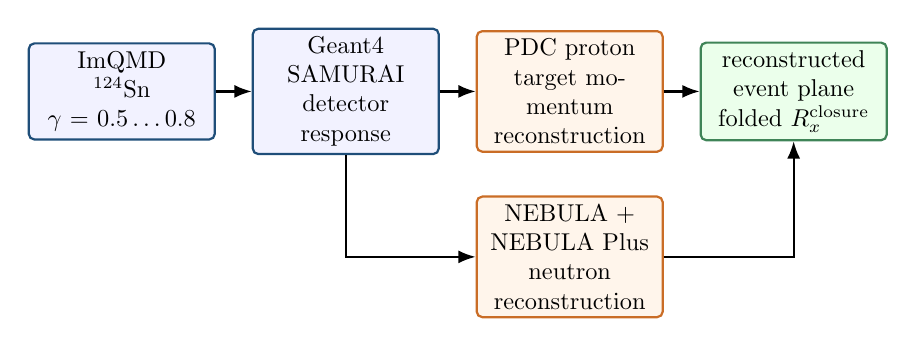
\begin{tikzpicture}[
    scale=0.88,
    transform shape,
    node distance=0.62cm and 0.52cm,
    box/.style={rectangle, rounded corners=2pt, draw=dpolblue, thick, align=center, minimum height=0.82cm, text width=2.45cm, fill=blue!5},
    reco/.style={rectangle, rounded corners=2pt, draw=dpolorange, thick, align=center, minimum height=0.82cm, text width=2.45cm, fill=orange!8},
    result/.style={rectangle, rounded corners=2pt, draw=dpolgreen, thick, align=center, minimum height=0.82cm, text width=2.45cm, fill=green!8},
    arrow/.style={-{Latex[length=2.2mm]}, thick}
  ]
    \node[box] (qmd) {ImQMD\\$^{124}$Sn\\$\gpar=0.5\ldots0.8$};
    \node[box, right=of qmd] (g4) {Geant4\\SAMURAI detector\\response};
    \node[reco, right=of g4] (pdc) {PDC proton\\target momentum\\reconstruction};
    \node[reco, below=of pdc] (nebula) {NEBULA +\\NEBULA Plus\\neutron reconstruction};
    \node[result, right=of pdc] (obs) {reconstructed\\event plane\\folded $\Rcl$};
    \draw[arrow] (qmd) -- (g4);
    \draw[arrow] (g4) -- (pdc);
    \draw[arrow] (g4) |- (nebula);
    \draw[arrow] (pdc) -- (obs);
    \draw[arrow] (nebula) -| (obs);
  \end{tikzpicture}

  \vspace{0.35cm}
  \begin{block}{Current closure scope}
    Fully reconstructed observable; truth-assisted event-quality selection;
    reco-defined px60 neutron fiducial.
  \end{block}
\end{frame}

\begin{frame}{Reconstruction Quality: Event Plane Is Measurable}
  \begin{columns}[T,onlytextwidth]
    \begin{column}{0.48\textwidth}
      \centering
      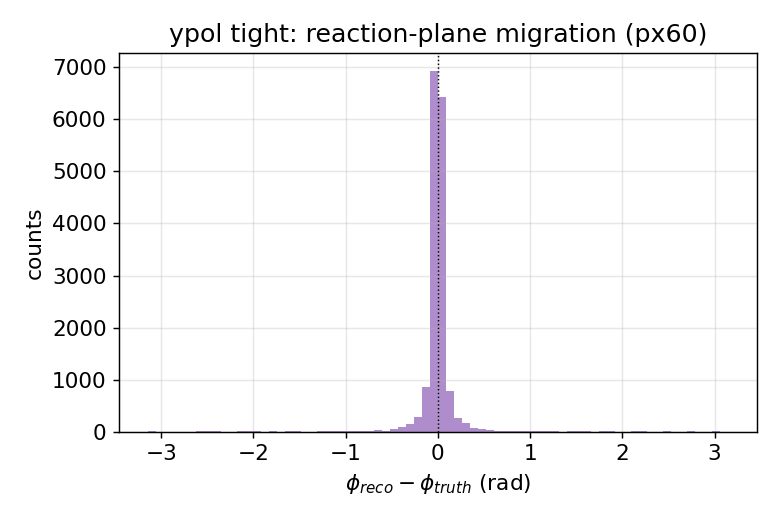
\includegraphics[width=0.96\linewidth]{dphi_reco_truth_ypol_tight_px60.png}

      \vspace{0.04cm}
      {\scriptsize y-pol tight px60: reconstructed minus truth event-plane angle.}
    \end{column}
    \begin{column}{0.52\textwidth}
      \scriptsize
      \begin{table}
        \centering
        \begin{tabular}{lccc}
          \toprule
          component & median & half-width & unit \\
          \midrule
          proton $\Delta p_x$ & $-0.79$ & $6.05$ & MeV/$c$ \\
          proton $\Delta p_y$ & $+0.51$ & $1.38$ & MeV/$c$ \\
          proton $\Delta p_z$ & $+1.59$ & $6.30$ & MeV/$c$ \\
          neutron $\Delta p_z$ & $-9.83$ & $8.72$ & MeV/$c$ \\
          \bottomrule
        \end{tabular}
      \end{table}
      \vspace{-0.12cm}
      Neutron transverse residuals are at the few-MeV/$c$ core scale in the
      accepted region; neutron $p_z$ from ToF is the larger momentum bias.
      \begin{block}{Why this matters for y-pol}
        \scriptsize
        The lab-fixed y-pol axis is related to each event's scattering plane by
        the reconstructed
        $\vec p_{T,p}^{\,\mathrm{reco}}+\vec p_{T,n}^{\,\mathrm{reco}}$.
      \end{block}
      \textbf{Closure implication:} reaction-plane migration gives a smaller
      correction in the $R$ ladder; it does not wash out the y-pol IVR ordering.
    \end{column}
  \end{columns}
\end{frame}

\begin{frame}{Why px60?}
  \begin{columns}[T,onlytextwidth]
    \begin{column}{0.58\textwidth}
      \centering
      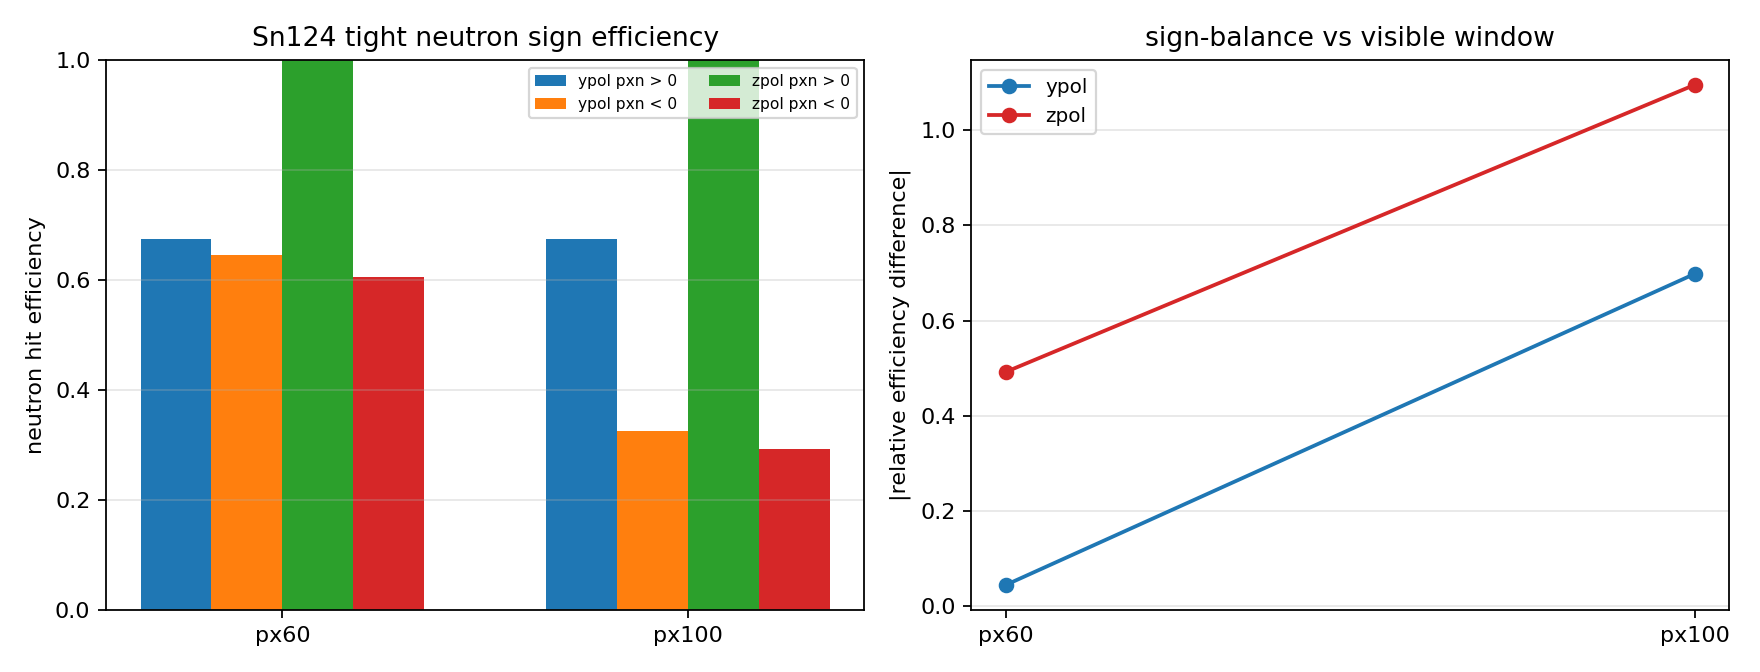
\includegraphics[width=\linewidth,height=0.70\textheight,keepaspectratio]{ypol_tight_neutron_efficiency_balance.png}
    \end{column}
    \begin{column}{0.42\textwidth}
      \scriptsize
      px60 is not chosen to remove all detector effects. It defines a region
      where the two neutron-$p_x$ signs have sufficiently balanced and nonzero
      efficiency.
      \[
        \epsilon(p_{x,n}>0)=0.678
      \]
      \[
        \epsilon(p_{x,n}<0)=0.644
      \]
      Relative imbalance: about $5\%$.
      \begin{block}{Why not px100?}
        \scriptsize
        The negative-$p_{x,n}$ branch has efficiency about $0.29$, producing a
        large sign-dependent distortion.
      \end{block}
      \textbf{Interpretation:} px60 is a controllable fiducial measurement, not
      an unfolded full-phase-space measurement.
    \end{column}
  \end{columns}
\end{frame}

\begin{frame}{Where Detector Folding Changes the Observable}
  \begin{columns}[T,onlytextwidth]
    \begin{column}{0.49\textwidth}
      \centering
      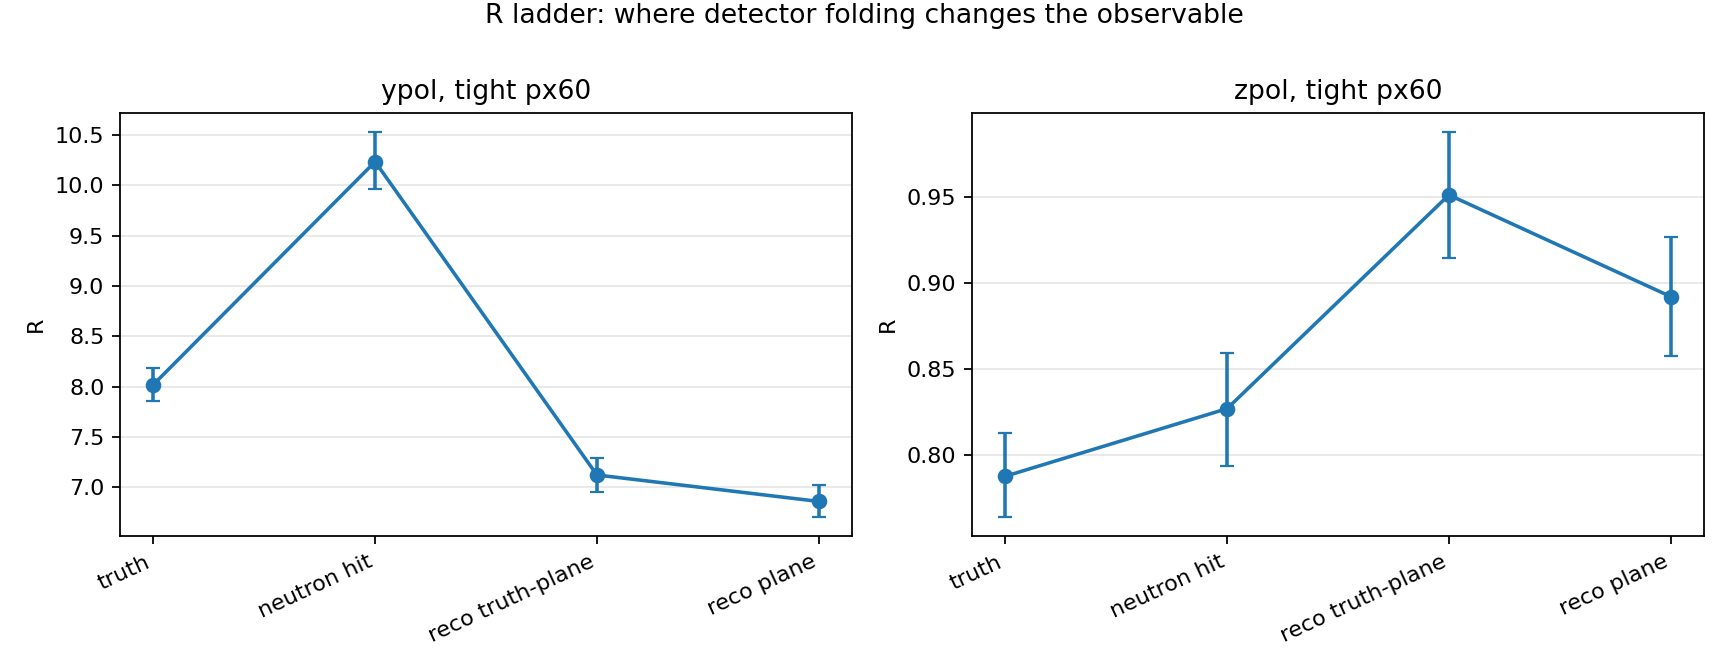
\includegraphics[width=\linewidth,height=0.70\textheight,keepaspectratio]{r_ladder_summary_tight_px60.png}
    \end{column}
    \begin{column}{0.51\textwidth}
      \scriptsize
      The ladder separates four stages:
      \begin{enumerate}
        \item truth fiducial,
        \item neutron-visible truth,
        \item reconstructed momenta with truth plane,
        \item fully reconstructed event plane.
      \end{enumerate}
      \begin{block}{Reading the ladder}
        \scriptsize
        The largest change comes from which neutron kinematics enter the
        visible phase space. Proton reconstruction is not the dominant
        bottleneck, and reaction-plane reconstruction adds a smaller shift.
      \end{block}
      \textbf{Observable consequence:} the absolute $R$ changes, while the
      $\gpar$ ordering remains.
    \end{column}
  \end{columns}
\end{frame}

\begin{frame}{Main Result: y-pol Gamma Ordering Survives}
  \centering
  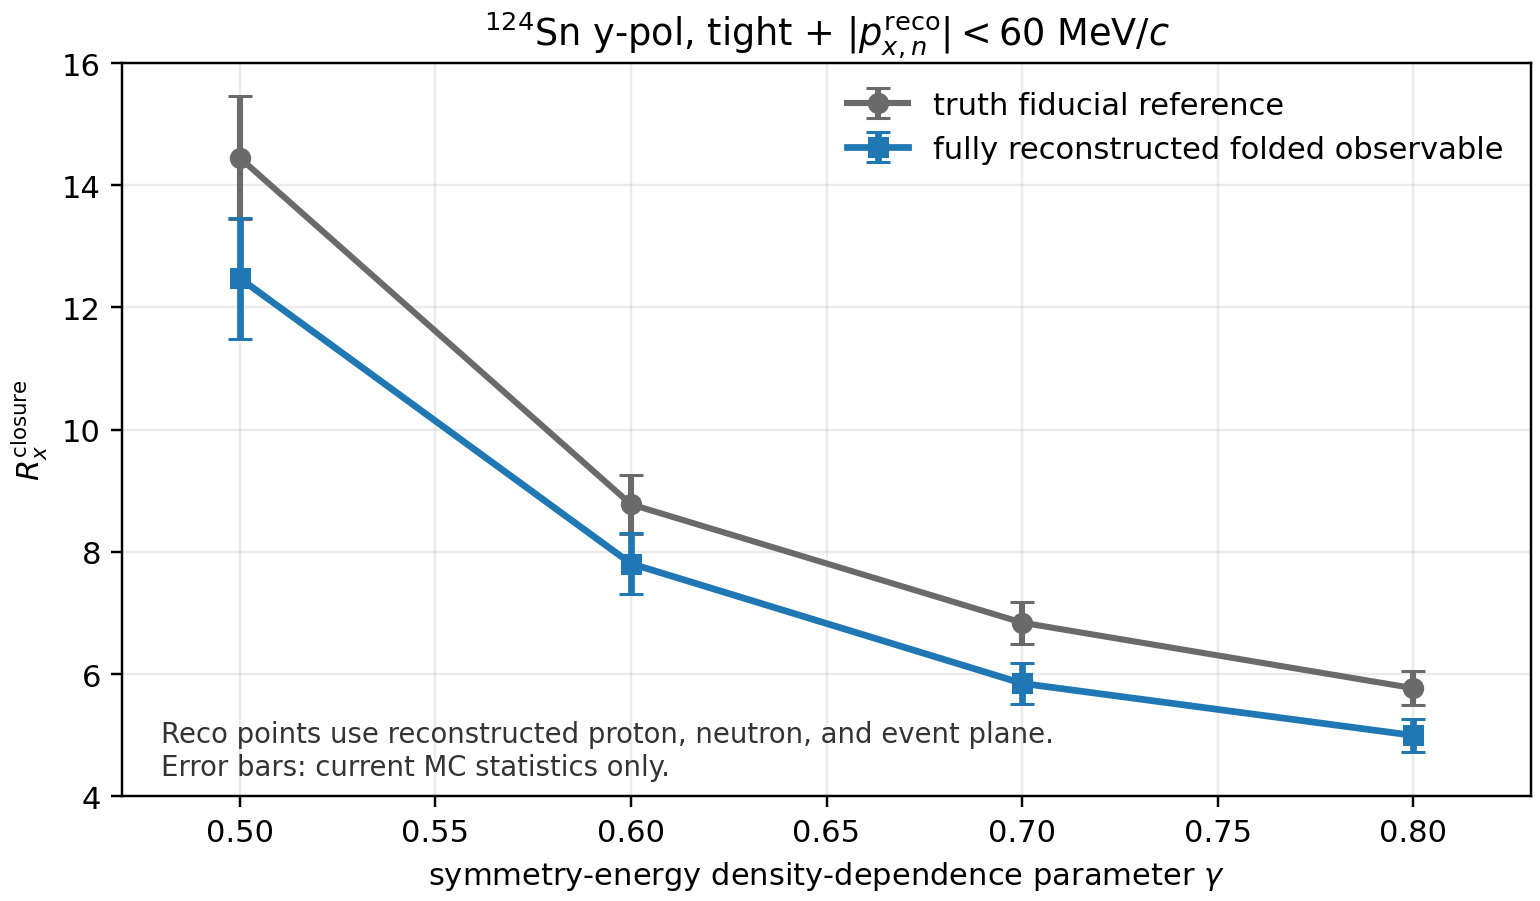
\includegraphics[height=0.66\textheight,keepaspectratio]{ypol_main_rx_closure.png}

  \vspace{0.02cm}
  \scriptsize
  $^{124}$Sn, y-pol, tight selected fiducial,
  $|p_{x,n}^{\mathrm{reco}}|<60$ MeV/$c$.

  \vspace{0.05cm}
  \textbf{Result:} the absolute ratio is changed by folding, but the monotonic
  $\gpar$ dependence remains visible after reconstructed proton, neutron, and
  reaction-plane determination.
\end{frame}

\begin{frame}{Statistics versus Systematics}
  \begin{columns}[T,onlytextwidth]
    \begin{column}{0.54\textwidth}
      \centering
      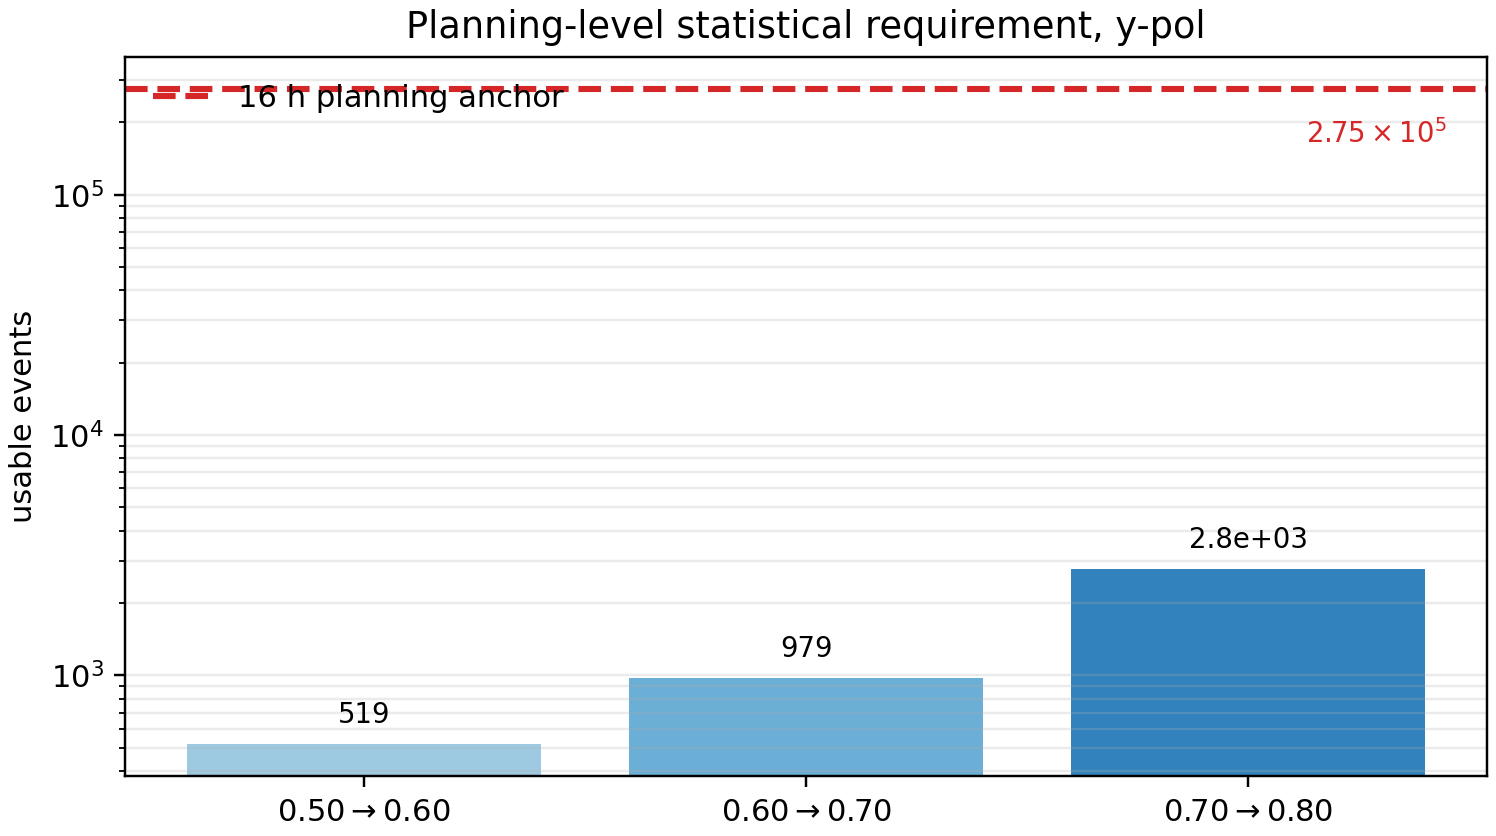
\includegraphics[width=\linewidth,height=0.67\textheight,keepaspectratio]{ypol_required_events.png}
    \end{column}
    \begin{column}{0.46\textwidth}
      \scriptsize
      Most difficult adjacent interval:
      $\gpar=0.7\to0.8$, with
      $N_{\mathrm{3\sigma}}\simeq2.8\times10^3$.

      Planning anchor, not a final beamtime guarantee:
      $10^7$ pps, 16 h, and 4.65\% detected-coincidence efficiency.

      Expected usable y-pol events:
      $N_{\mathrm{usable}}\simeq2.75\times10^5$.
      \begin{block}{Implication}
        \scriptsize
        Statistics are not expected to be the main limitation. Detector
        response, neutron efficiency, polarization knowledge, backgrounds, and
        model systematics will dominate.
      \end{block}
    \end{column}
  \end{columns}
\end{frame}

\begin{frame}{What Remains before Experimental Analysis?}
  \small
  \begin{enumerate}
    \item Replace truth-assisted event-quality cuts with reco-only cuts.
    \item Quantify selection efficiency, purity, and migration.
    \item Propagate $p_{yy}$ monitoring uncertainty into $R_x(\gpar)$.
    \item Validate neutron threshold, $T_0$, cross-talk, fake neutron,
      background, and detector-response systematics.
  \end{enumerate}
  \vspace{0.18cm}
  \begin{block}{Highest priority}
    Reco-only cut closure: show that the same y-pol $\gpar$ ordering survives
    when every experimental selection is defined using reconstructed quantities.
  \end{block}
  \begin{block}{Pseudo-data program}
    Perform closure tests under detector and model variations before quoting an
    experimental uncertainty budget.
  \end{block}
\end{frame}

\begin{frame}{Preparation Timeline}
  \scriptsize
  \begin{columns}[T,totalwidth=\textwidth]
    \begin{column}{0.47\textwidth}
      \begin{block}{Analysis readiness}
        \begin{itemize}
          \item Jul--Aug 2026: reco-only cut closure.
          \item Sep 2026: detector-response variations.
          \item Sep--Oct 2026: pseudo-data tests.
          \item Oct 2026: frozen folded-observable definition.
        \end{itemize}
      \end{block}
      \begin{block}{Experiment readiness}
        \begin{itemize}
          \item Nov--Dec 2026: polarimeter checklist.
          \item Dec 2026: detector-run checklist.
          \item Jan--Feb 2027: final run plan and beam request.
        \end{itemize}
      \end{block}
    \end{column}
    \begin{column}{0.47\textwidth}
      \begin{block}{Requested beam period}
        Target physics beam: \textbf{May 2027}.
      \end{block}
      \begin{block}{Status}
        This is a planning target, not an approved beamtime assignment.  The
        final month must follow the RIBF/SAMURAI machine and PAC schedule.
      \end{block}
      \begin{block}{Decision gate}
        The run request should follow reco-only closure and a first detector
        systematic budget.
      \end{block}
    \end{column}
  \end{columns}
\end{frame}

\begin{frame}{Summary}
  \small
  \begin{enumerate}
    \item $^{124}$Sn y-pol provides a strong IVR-sensitive observable.
    \item The $\gpar$-dependent ordering survives reconstructed proton,
      reconstructed neutron, and reconstructed event-plane determination in
      the px60 fiducial region.
    \item The primary experimental strategy is folded data versus identically
      folded model predictions.
    \item A y-pol run is sufficient to demonstrate the IVR measurement concept;
      z-pol can be added after successful commissioning.
  \end{enumerate}
  \vspace{0.2cm}
  \begin{block}{Bottom line}
    The current result demonstrates detector-level observability, not yet a
    complete experimental uncertainty budget.
  \end{block}
\end{frame}

\begin{frame}
  \centering
  \Huge Thanks

  \vspace{0.6cm}
  \Large Questions?
\end{frame}

\appendix
\setbeamertemplate{footline}{}
\section*{Backup}

\begin{frame}{Backup Roadmap}
  \small
  \begin{columns}[T,onlytextwidth]
    \begin{column}{0.50\textwidth}
      \begin{itemize}
        \item A: Observable and folding definitions
        \item B: y-pol reconstruction diagnostics
        \item C: neutron acceptance and px-window studies
        \item D: gamma sensitivity and statistics
      \end{itemize}
    \end{column}
    \begin{column}{0.50\textwidth}
      \begin{itemize}
        \item E: target and polarization extensions
        \item F: polarization monitoring
        \item G: limitations and future closure
      \end{itemize}
    \end{column}
  \end{columns}
\end{frame}

\begin{frame}{Backup A: Observable Definitions}
  \small
  \[
    \phi_{\mathrm{truth/reco}} =
    \operatorname{atan2}(p_{y,p}+p_{y,n},\,p_{x,p}+p_{x,n})
  \]
  \[
    \Delta p_x^{\mathrm{rot}} =
    p_{x,p}^{\mathrm{rot}}-p_{x,n}^{\mathrm{rot}},
    \qquad
    R_x=\frac{N(\Delta p_x^{\mathrm{rot}}>0)}
             {N(\Delta p_x^{\mathrm{rot}}<0)} .
  \]
  \[
    \Ax=\frac{N_+-N_-}{N_++N_-}
       =\frac{R_x-1}{R_x+1}.
  \]
  \begin{block}{Naming in this talk}
    Truth, folded, reconstructed, and unfolded observables are different
    objects.  The main y-pol result is $\Rcl$, a detector-level closure
    observable in a reconstructed fiducial region.
  \end{block}
\end{frame}

\begin{frame}{Backup A: Folding and Unfolding Vocabulary}
  \small
  \[
    N_{\mathrm{reco},j}=\sum_iK_{ji}N_{\mathrm{true},i}+b_j .
  \]
  \begin{itemize}
    \item truth: generator-level kinematics after physics selection.
    \item folded: model events passed through detector response and
      reconstruction.
    \item reco: reconstructed variables used exactly as experimental data would
      be used.
    \item unfolded: estimator of truth after response inversion, requiring
      regularization and closure.
  \end{itemize}
  \begin{block}{Current cut state}
    y-pol tight event-quality selection is still truth-assisted; the px60
    neutron fiducial is reconstructed.  This is why the result is called a
    detector-level closure test.
  \end{block}
\end{frame}

\begin{frame}{Backup B: Proton and Neutron Residuals}
  \begin{columns}[T,onlytextwidth]
    \begin{column}{0.50\textwidth}
      \centering
      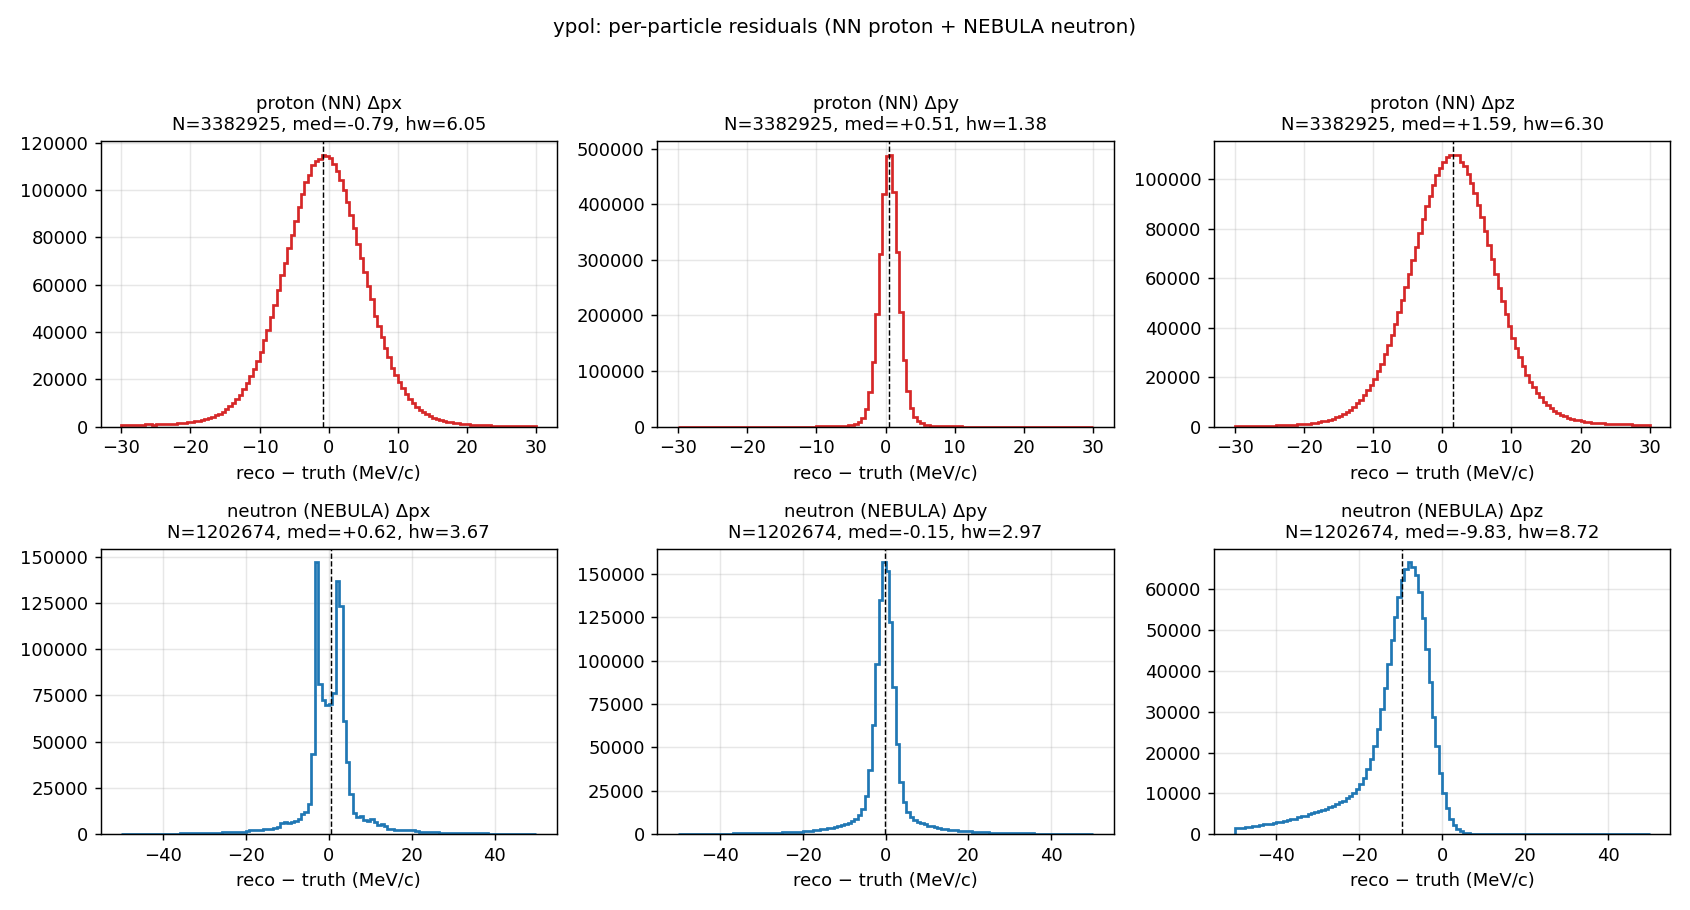
\includegraphics[width=\linewidth]{residuals_per_particle_ypol.png}
    \end{column}
    \begin{column}{0.50\textwidth}
      \centering
      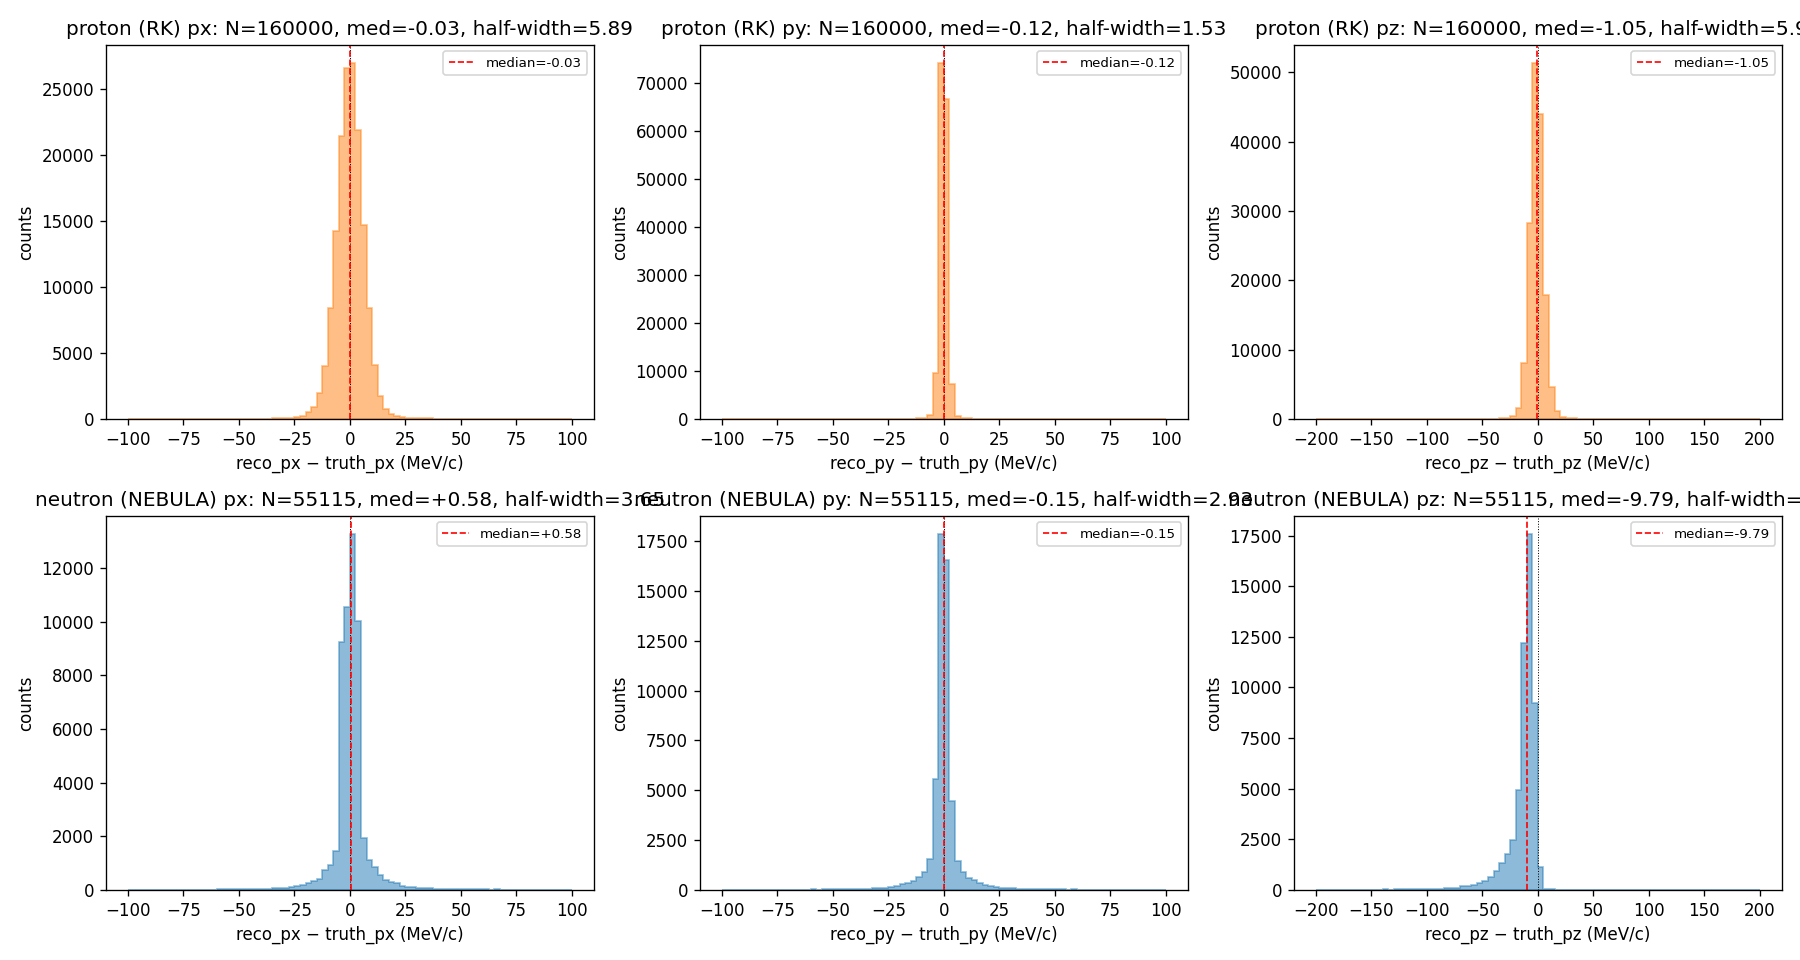
\includegraphics[width=\linewidth]{reco_residuals_per_particle.png}
    \end{column}
  \end{columns}
  \vspace{0.08cm}
  \scriptsize
  Left: NN breakup diagnostic. Right: earlier RK+NEBULA y-pol full-reco study.
  Residual half-width and RMSE are distinct quantities; tails matter for RMSE.
\end{frame}

\begin{frame}{Backup B: Reconstructed Event Plane}
  \begin{columns}[T,onlytextwidth]
    \begin{column}{0.52\textwidth}
      \centering
      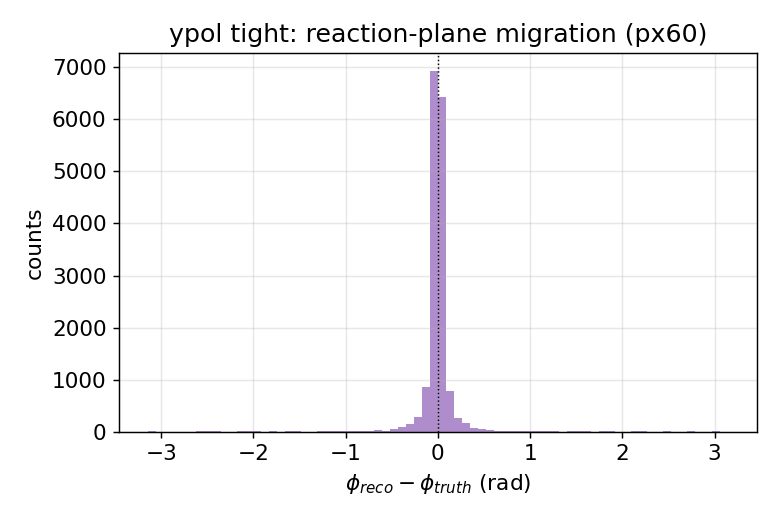
\includegraphics[width=\linewidth]{dphi_reco_truth_ypol_tight_px60.png}
    \end{column}
    \begin{column}{0.48\textwidth}
      \centering
      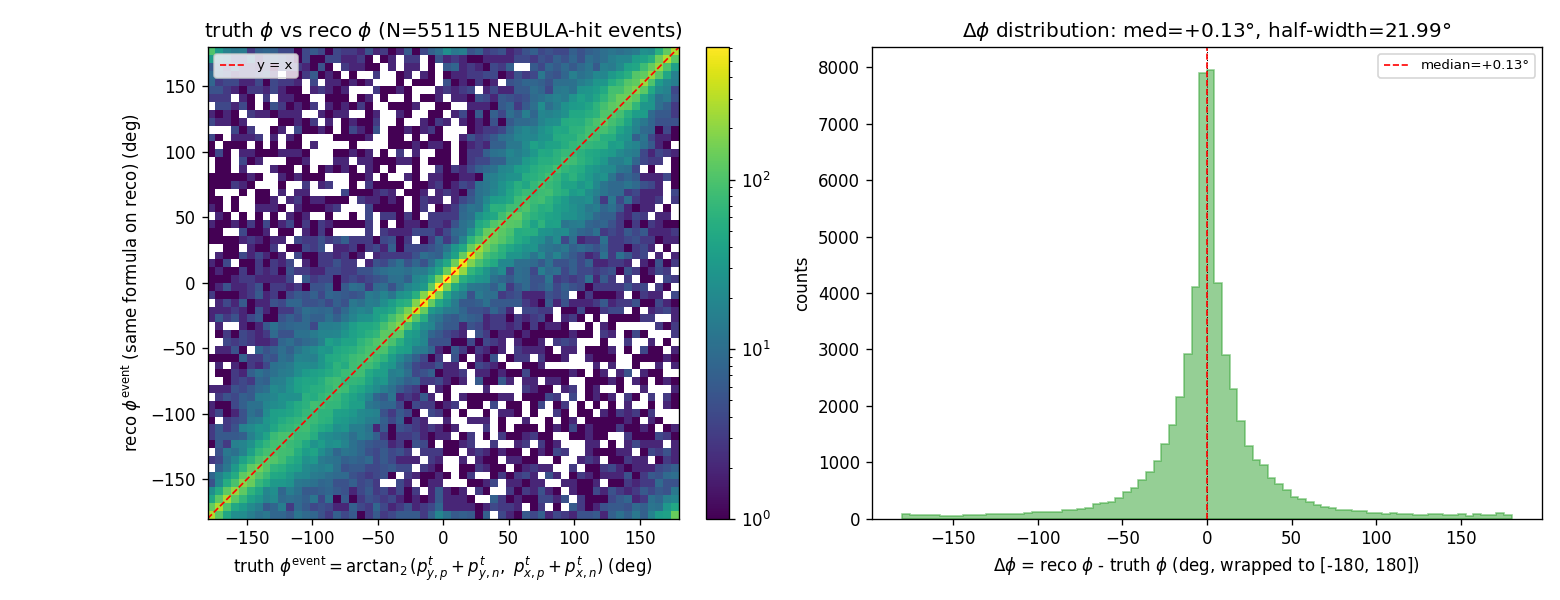
\includegraphics[width=\linewidth]{truth_phi_vs_reco_phi.png}
    \end{column}
  \end{columns}
  \vspace{0.08cm}
  \scriptsize
  Reaction-plane reconstruction broadens the observable but is not the largest
  change in the R ladder for tight px60.
\end{frame}

\begin{frame}{Backup B: RK vs NN Proton Cross-Check}
  \begin{columns}[T,onlytextwidth]
    \begin{column}{0.54\textwidth}
      \centering
      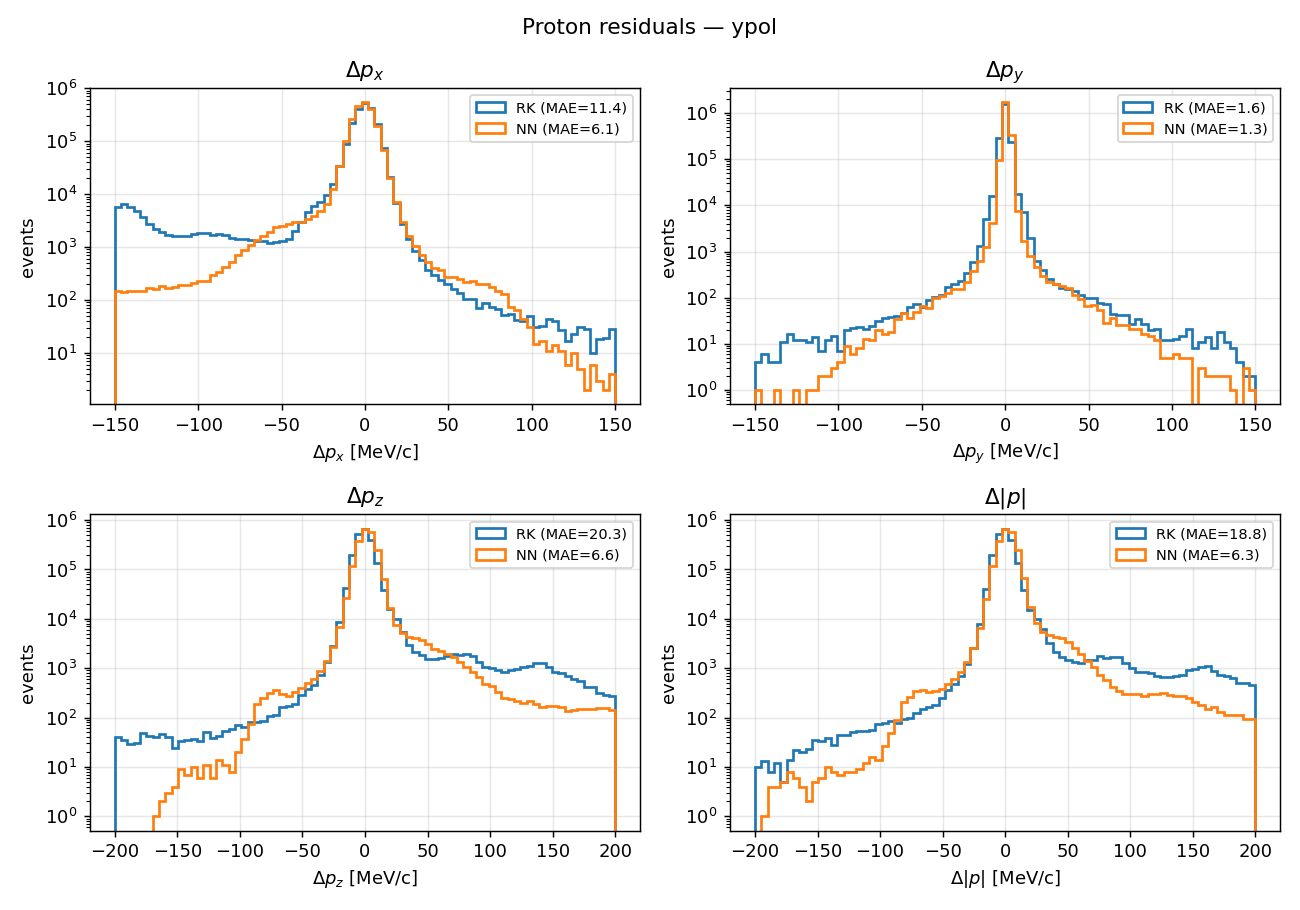
\includegraphics[width=\linewidth]{proton_residuals_ypol.png}
    \end{column}
    \begin{column}{0.46\textwidth}
      \scriptsize
      Strict RK--NN comparison is available on the common configuration without
      NEBULA Plus.
      \begin{table}
        \centering
        \begin{tabular}{lrr}
          \toprule
          y-pol metric & RK & NN \\
          \midrule
          $\Delta p_x$ half-width & 5.86 & 6.01 \\
          $\Delta p_x$ RMSE & 39.7 & 13.3 \\
          $\Delta p_z$ half-width & 5.88 & 6.25 \\
          $\Delta p_z$ RMSE & 87.8 & 15.7 \\
          \bottomrule
        \end{tabular}
      \end{table}
      Proton reconstruction has been cross-checked against RK and is not the
      dominant source of the observable shift.
    \end{column}
  \end{columns}
\end{frame}

\begin{frame}{Backup B: NN Proton Backend}
  \small
  \begin{columns}[T,onlytextwidth]
    \begin{column}{0.48\textwidth}
      \begin{block}{Inputs}
        PDC1/PDC2 hit positions:
        \[
          (x_1,y_1,z_1,x_2,y_2,z_2).
        \]
      \end{block}
      \begin{block}{Outputs}
        Target-frame proton momentum:
        \[
          (p_x,p_y,p_z)_{\mathrm{target}}.
        \]
      \end{block}
    \end{column}
    \begin{column}{0.52\textwidth}
      \begin{itemize}
        \item MLP backend used through the canonical reconstruction CLI.
        \item Training domain covers the breakup kinematics used here.
        \item NN has comparable core resolution to RK and smaller catastrophic
          tails in the common-geometry comparison.
      \end{itemize}
    \end{column}
  \end{columns}
\end{frame}

\begin{frame}{Backup C: px60, px80, px100}
  \begin{columns}[T,onlytextwidth]
    \begin{column}{0.33\textwidth}
      \centering
      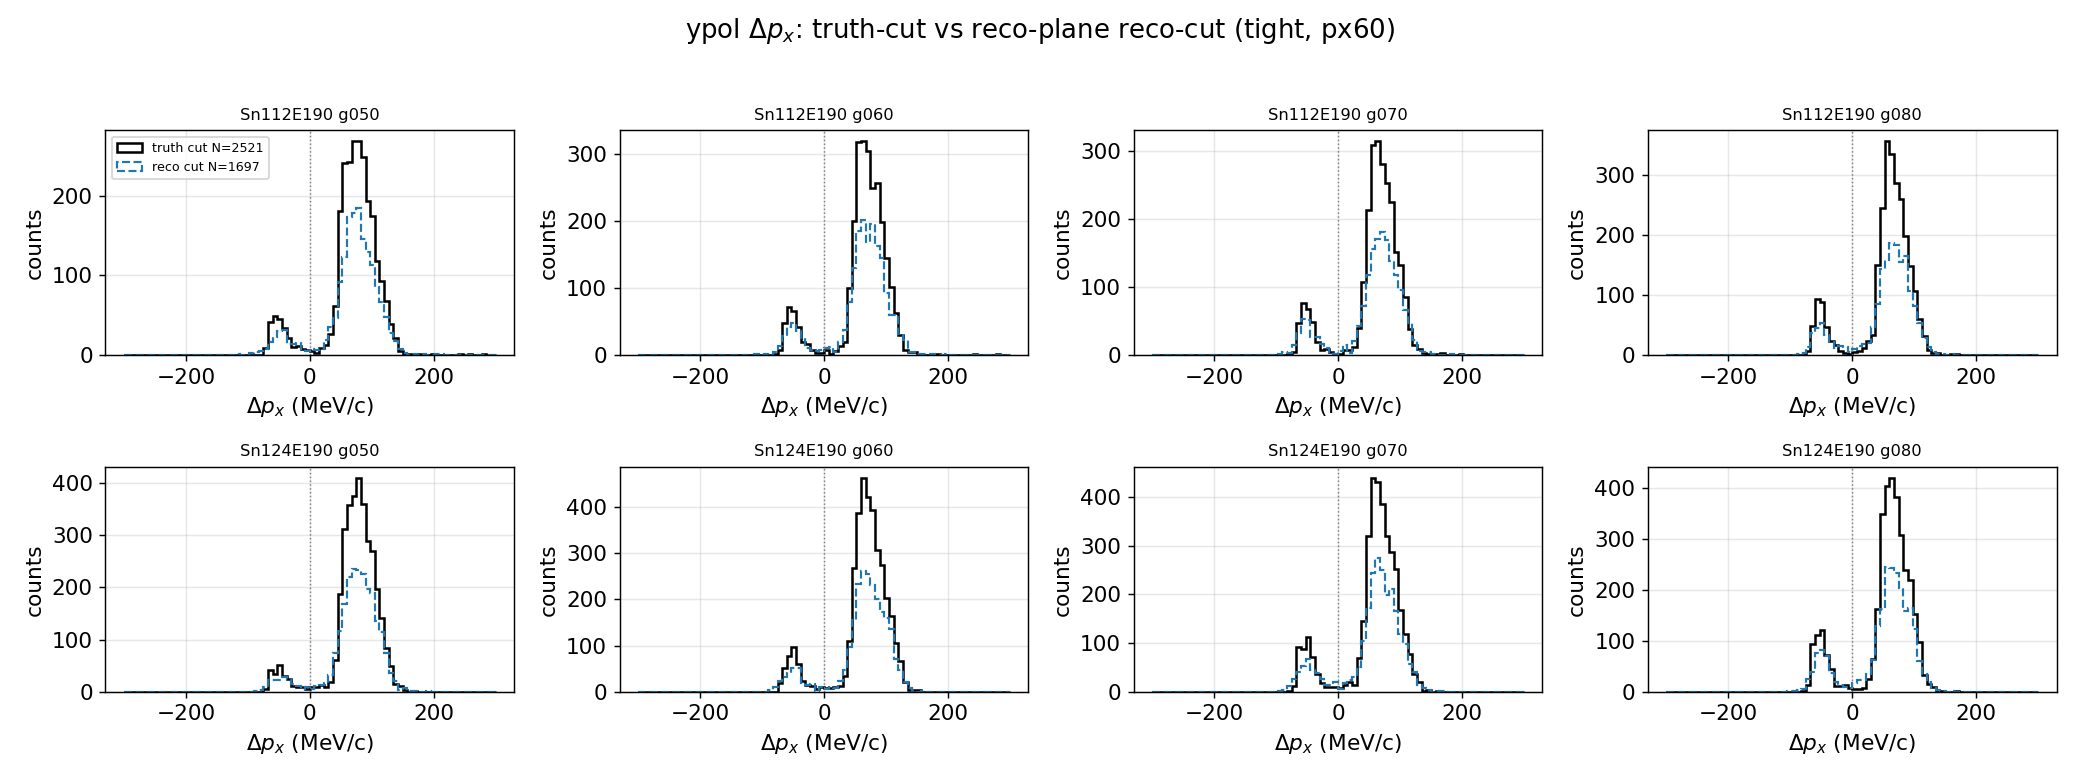
\includegraphics[width=\linewidth]{px_diff_hist_ypol_tight_reco_plane_px60.png}
      {\scriptsize px60}
    \end{column}
    \begin{column}{0.33\textwidth}
      \centering
      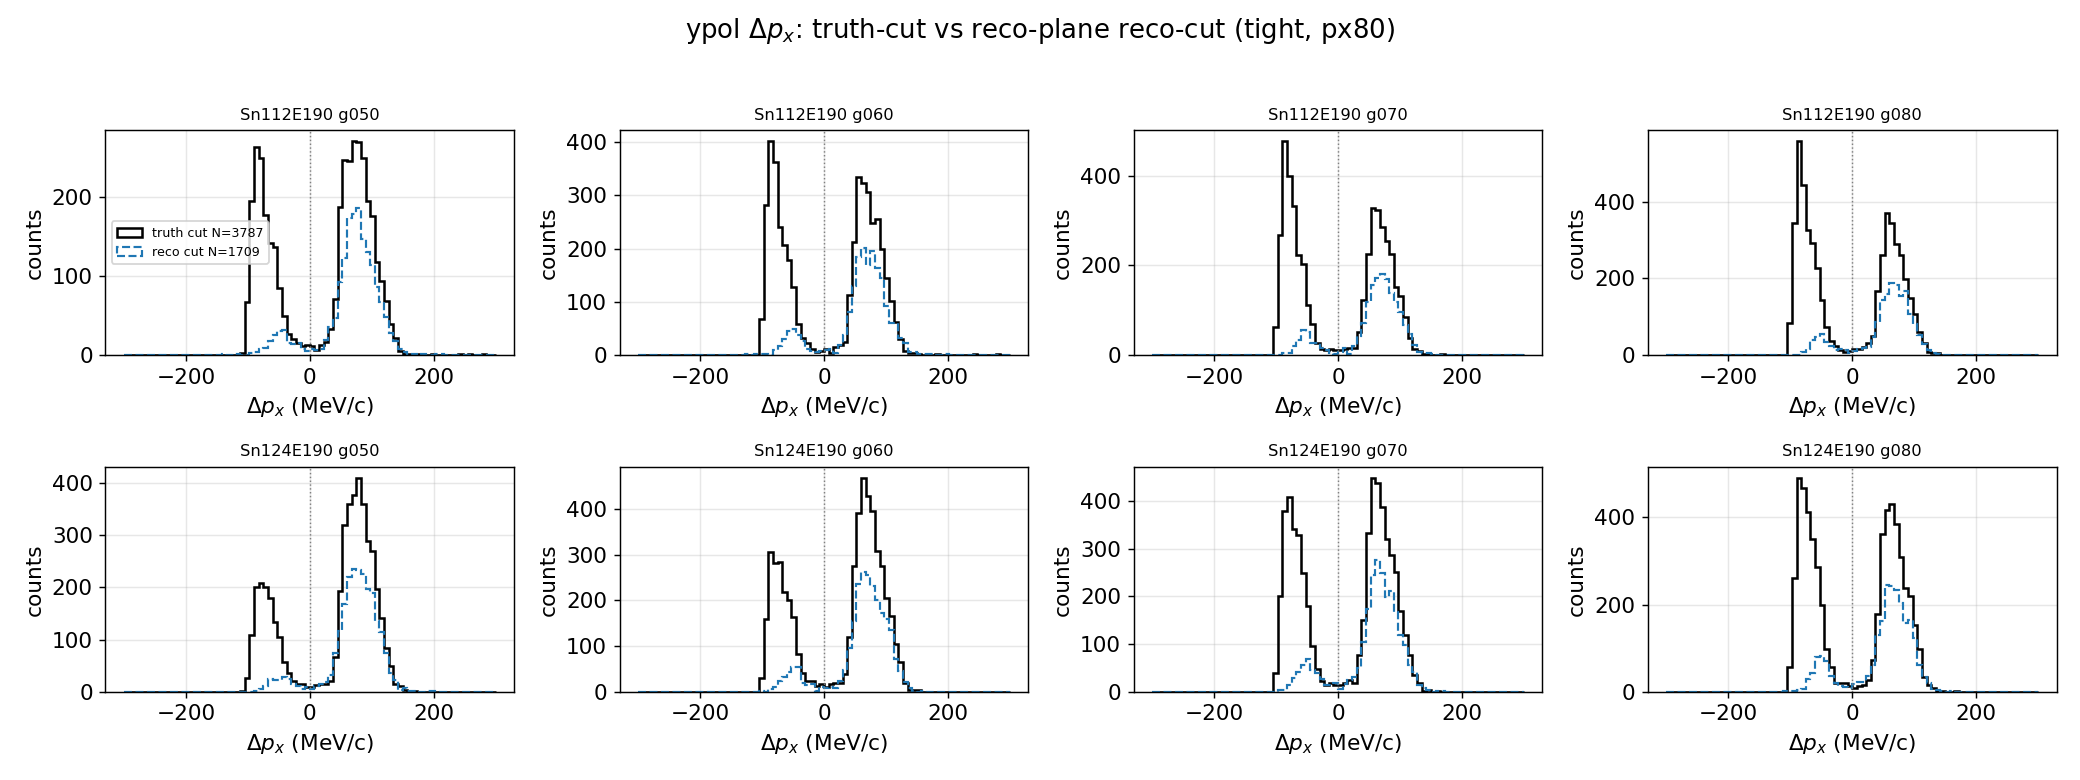
\includegraphics[width=\linewidth]{px_diff_hist_ypol_tight_reco_plane_px80.png}
      {\scriptsize px80}
    \end{column}
    \begin{column}{0.33\textwidth}
      \centering
      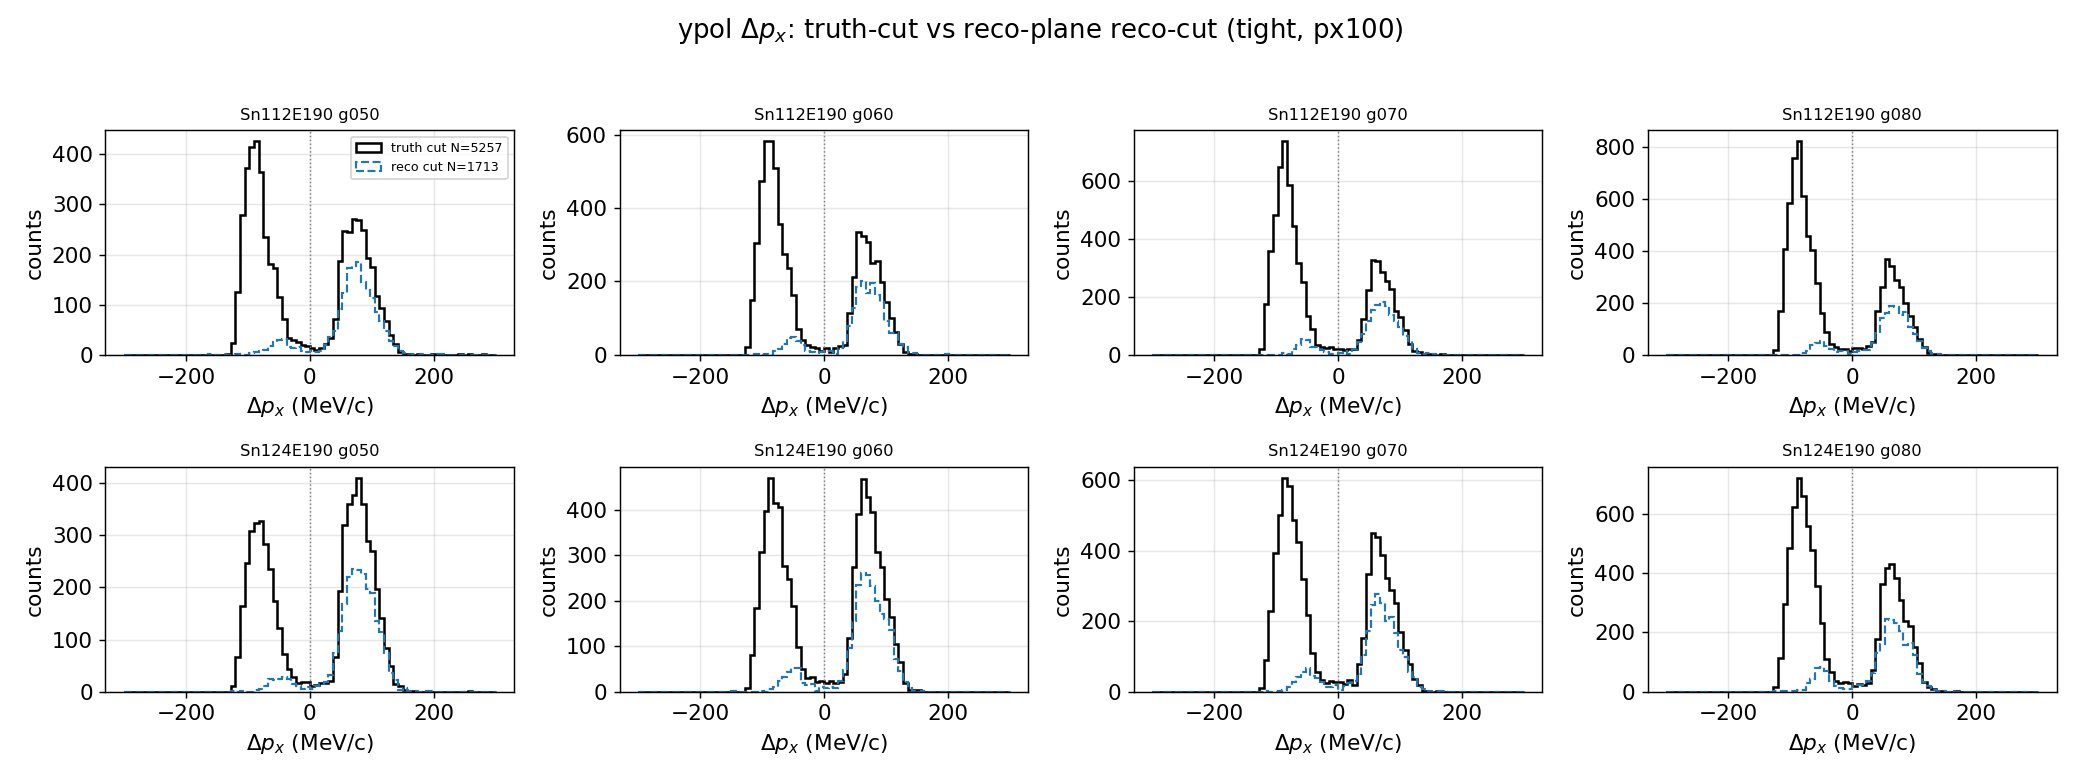
\includegraphics[width=\linewidth]{px_diff_hist_ypol_tight_reco_plane_px100.png}
      {\scriptsize px100}
    \end{column}
  \end{columns}
  \vspace{0.08cm}
  \scriptsize
  px80 improves over px100, but px60 removes most of the low-efficiency
  negative-$p_{x,n}$ branch.
\end{frame}

\begin{frame}{Backup C: 1D Neutron Efficiency}
  \centering
  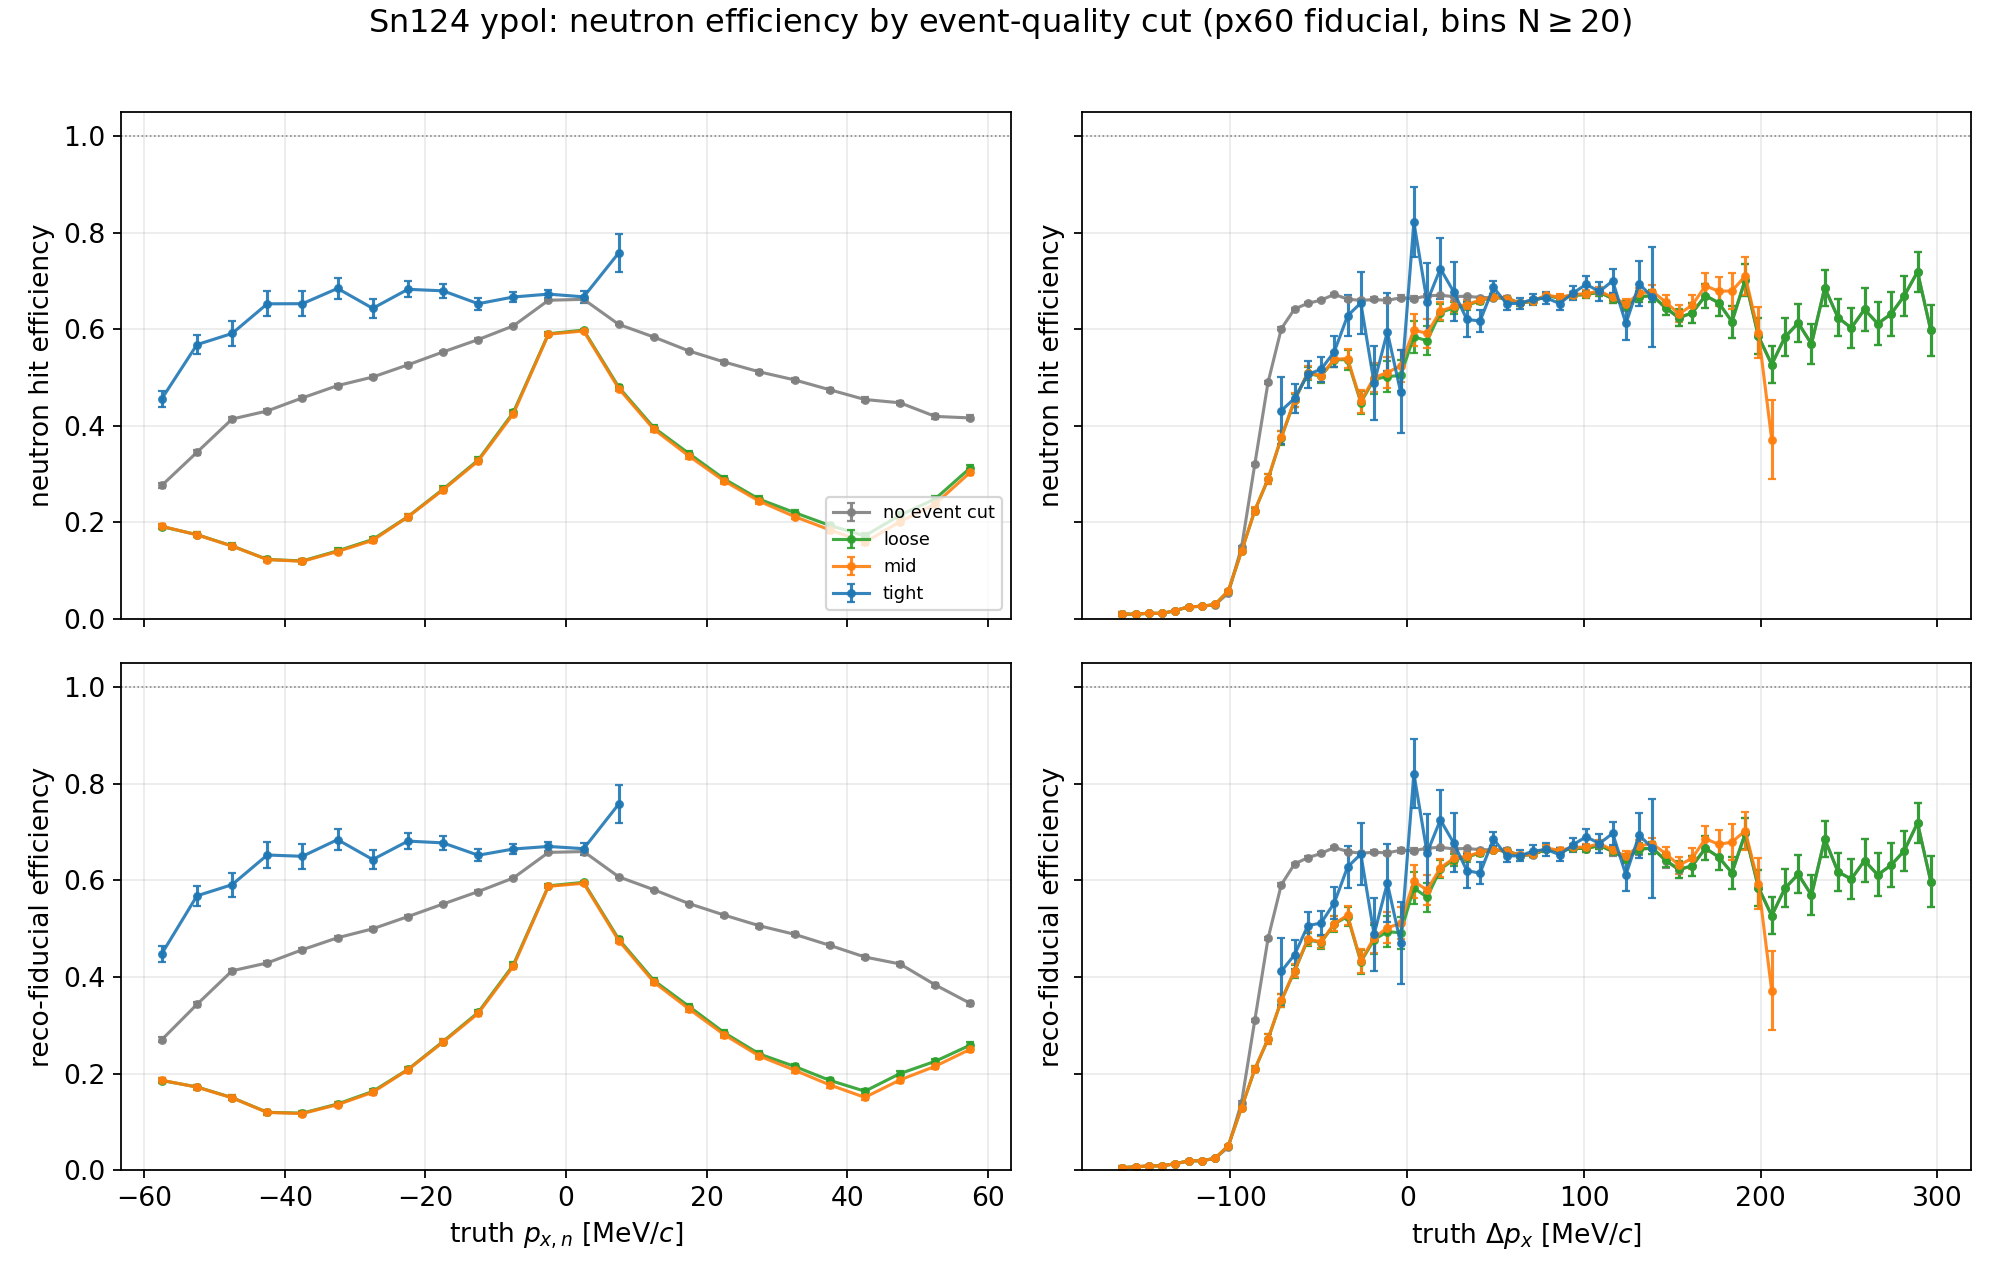
\includegraphics[height=0.68\textheight,keepaspectratio]{neutron_efficiency_1d_by_cut_ypol.png}

  \vspace{0.08cm}
  \scriptsize
  Efficiency shape is similar across event-quality cuts; the cut mainly changes
  which phase-space region is populated.
\end{frame}

\begin{frame}{Backup C: 2D Neutron Efficiency}
  \centering
  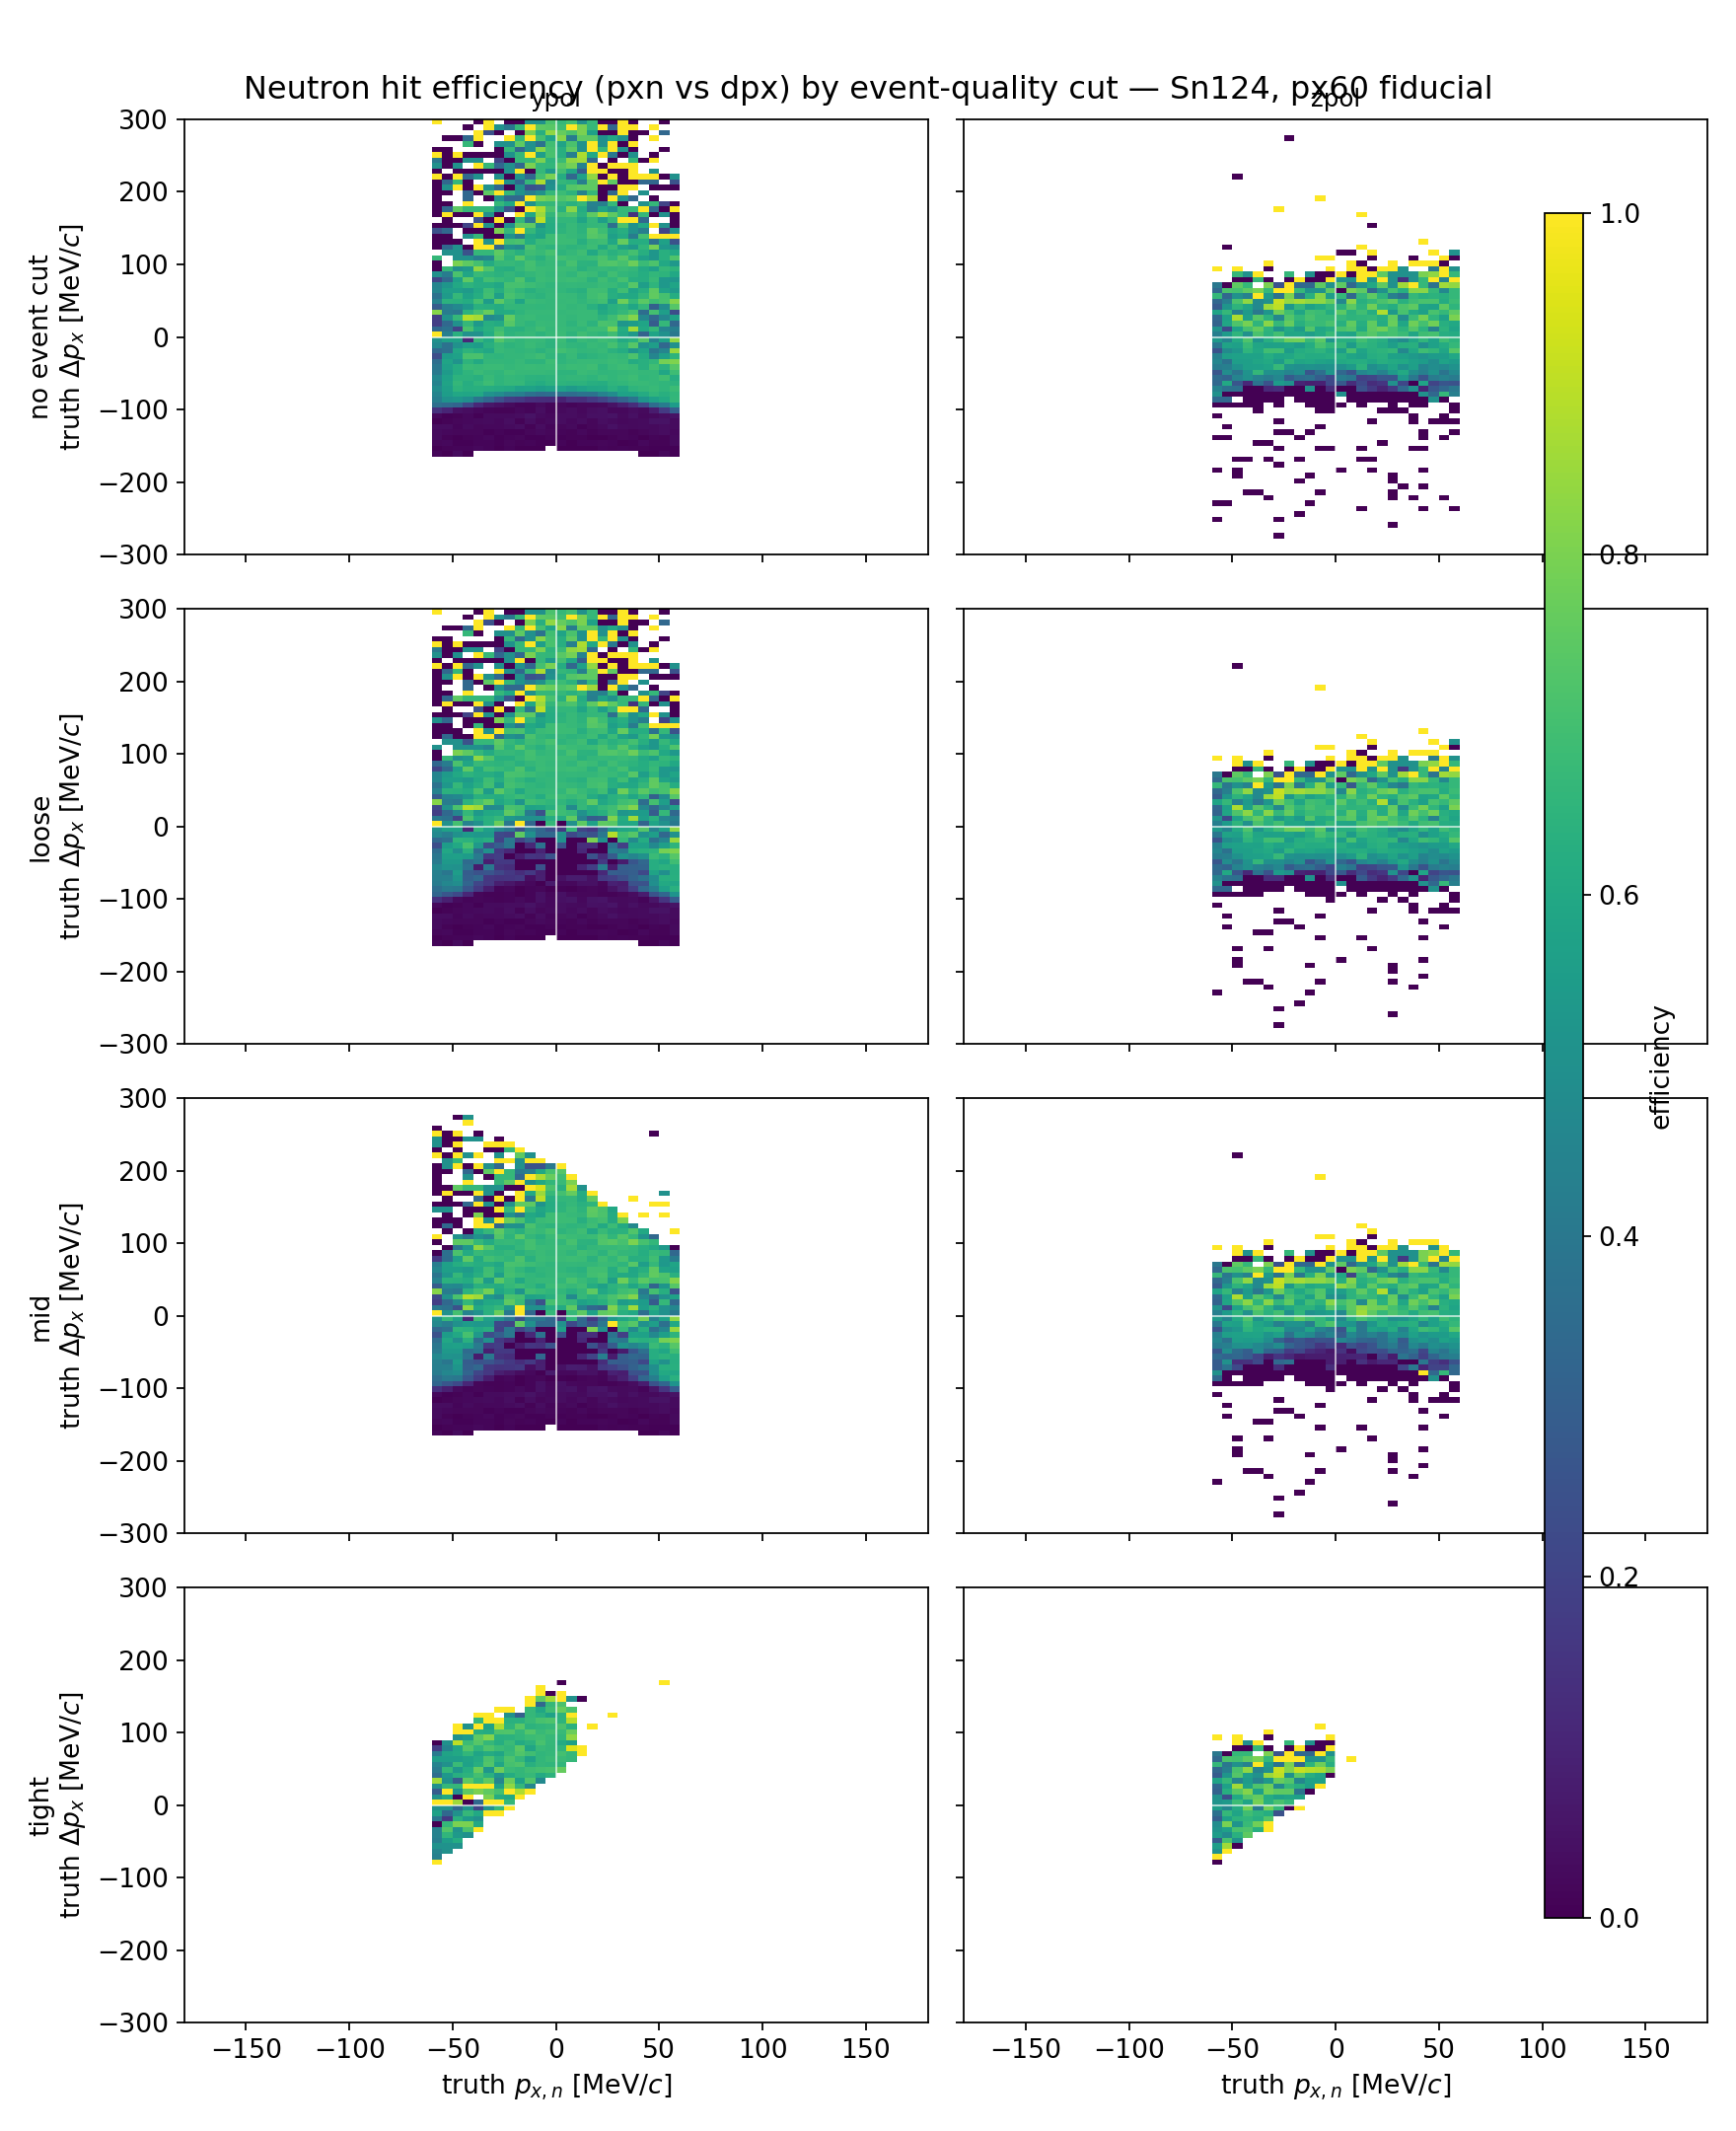
\includegraphics[height=0.66\textheight,keepaspectratio]{neutron_efficiency_2d_pxn_vs_dpx_by_cut.png}

  \vspace{0.08cm}
  \scriptsize
  The response is not uniform in $(p_{x,n},\Delta p_x)$; this is why folded
  comparison is the primary strategy.
\end{frame}

\begin{frame}{Backup C: No-Fiducial Efficiency Landscape}
  \centering
  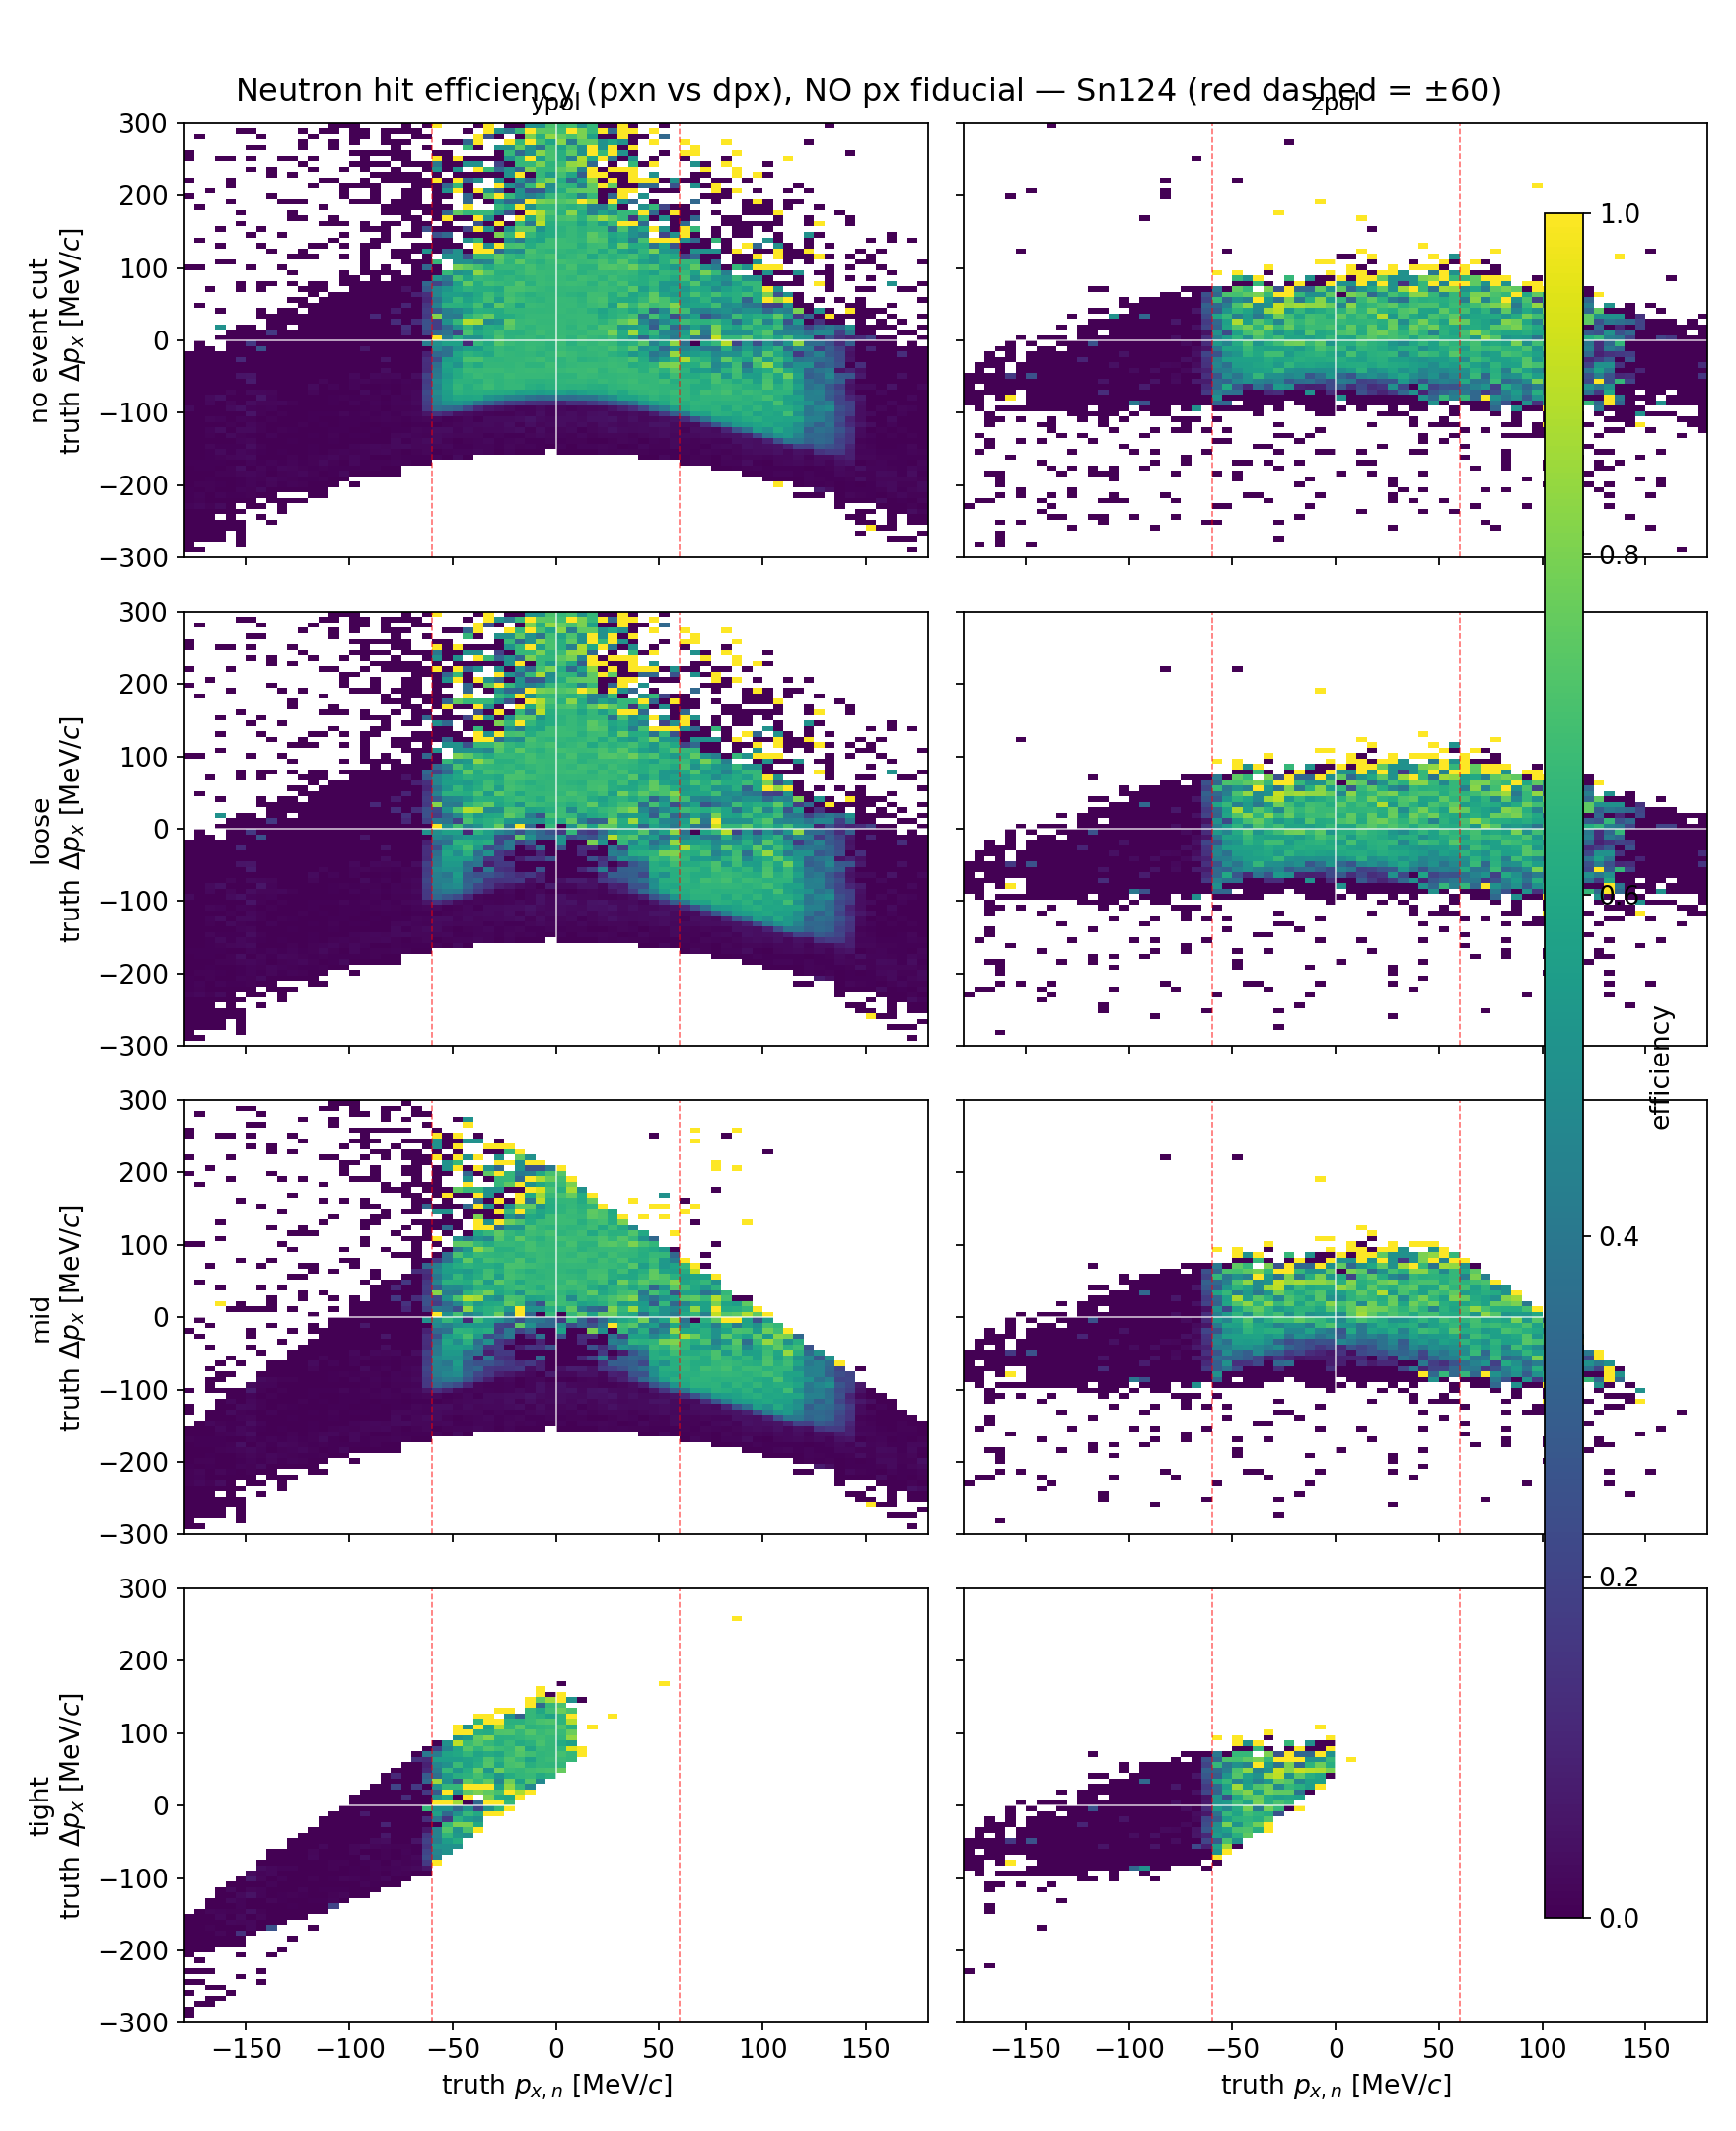
\includegraphics[height=0.66\textheight,keepaspectratio]{neutron_efficiency_2d_pxn_vs_dpx_nofiducial.png}

  \vspace{0.08cm}
  \scriptsize
  The red guide lines mark $\pm60$ MeV/$c$.  Near-zero-efficiency regions make a
  simple $1/\epsilon$ correction or raw unfolding unstable.
\end{frame}

\begin{frame}{Backup C: Sign Migration}
  \centering
  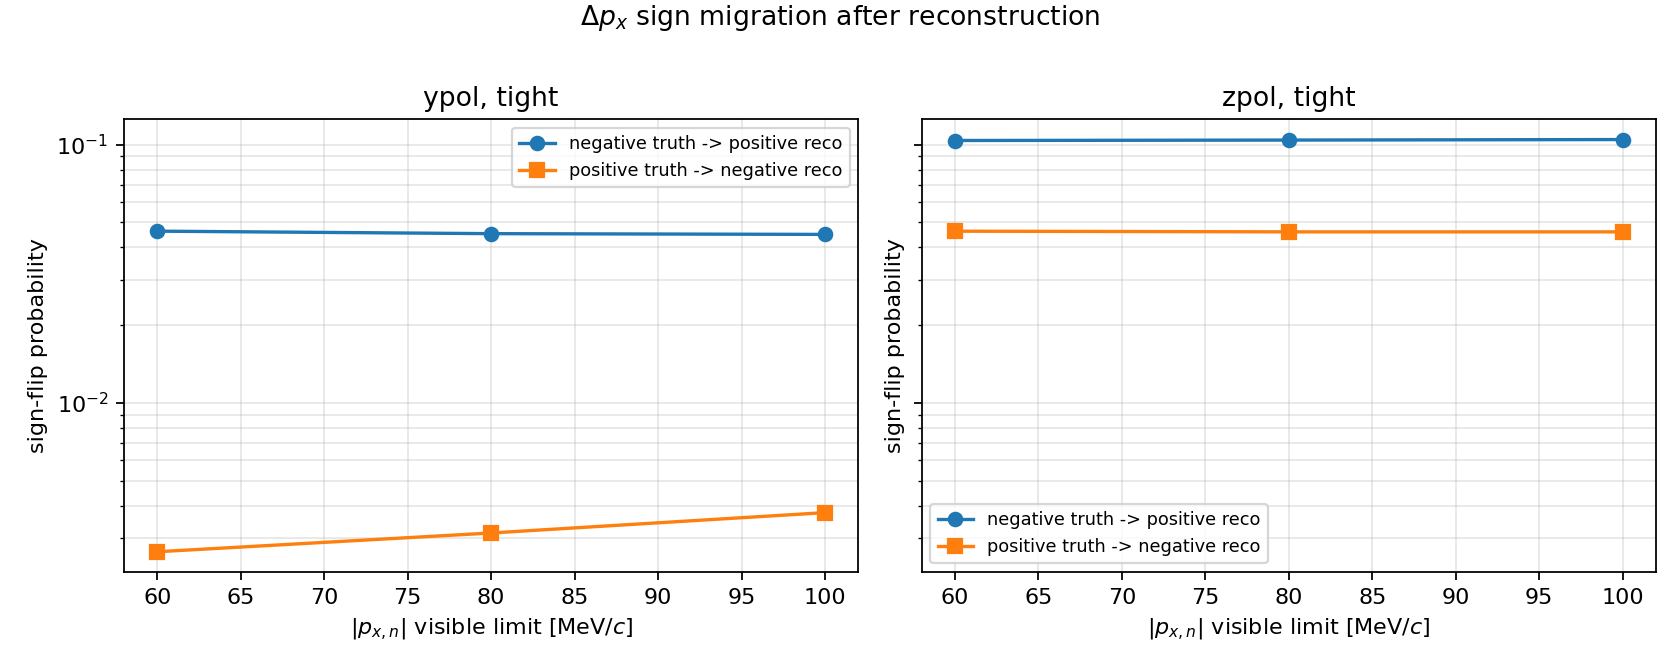
\includegraphics[width=0.72\linewidth]{sign_migration_summary_tight.png}

  \vspace{0.08cm}
  \scriptsize
  In y-pol tight px60, $\Delta p_x$ sign migration is small compared with the
  neutron visibility effect.
\end{frame}

\begin{frame}{Backup C: Response Matrices}
  \centering
  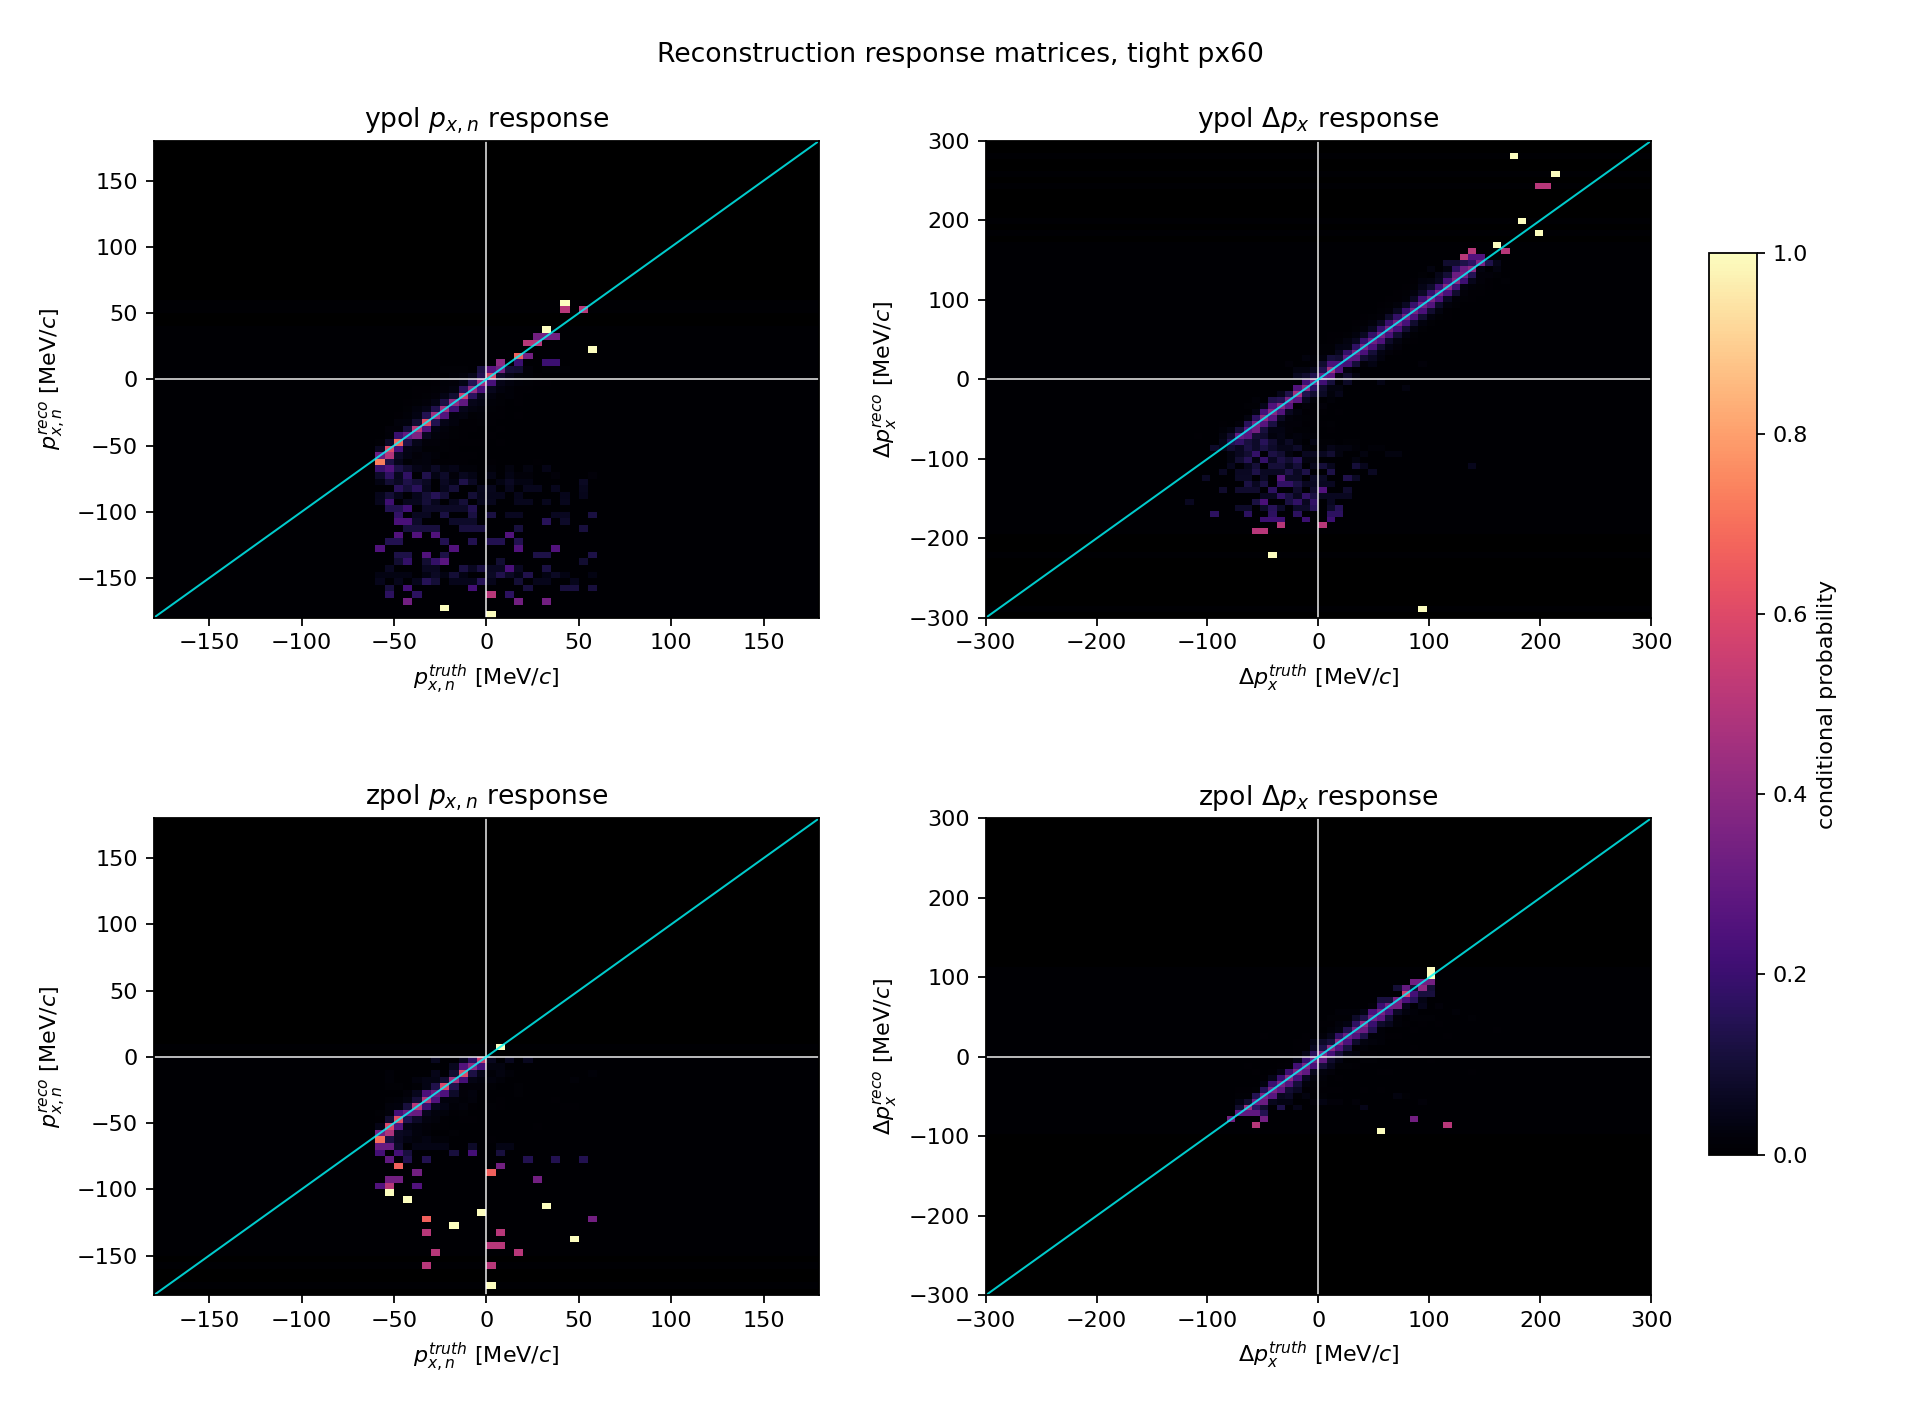
\includegraphics[height=0.64\textheight,keepaspectratio]{response_matrices_tight_px60.png}

  \vspace{0.08cm}
  \scriptsize
  Response matrices are useful for closure and possible unfolding, but the main
  result avoids relying on an unstable inverse problem.
\end{frame}

\begin{frame}{Backup D: Full y-pol Numbers}
  \scriptsize
  \begin{table}
    \centering
    \begin{tabular}{lrrrrr}
      \toprule
      $\gpar$ & $N_+$ & $N_-$ & $\Rcl\pm\sigma_{\mathrm{MC}}$ & $\Ax$ & $N_{\mathrm{used}}$ \\
      \midrule
      0.5 & 2134 & 171 & $12.48\pm0.99$ & 0.852 & 2305 \\
      0.6 & 2147 & 275 & $\phantom{0}7.81\pm0.50$ & 0.773 & 2422 \\
      0.7 & 2093 & 358 & $\phantom{0}5.85\pm0.33$ & 0.708 & 2451 \\
      0.8 & 1948 & 390 & $\phantom{0}4.99\pm0.28$ & 0.666 & 2338 \\
      \bottomrule
    \end{tabular}
  \end{table}
  \begin{block}{Meaning}
    These are folded reco-plane values for $^{124}$Sn y-pol tight px60, not
    truth-level asymmetries.  Uncertainties are current MC statistical only.
  \end{block}
\end{frame}

\begin{frame}{Backup D: Bounded Asymmetry Cross-Check}
  \centering
  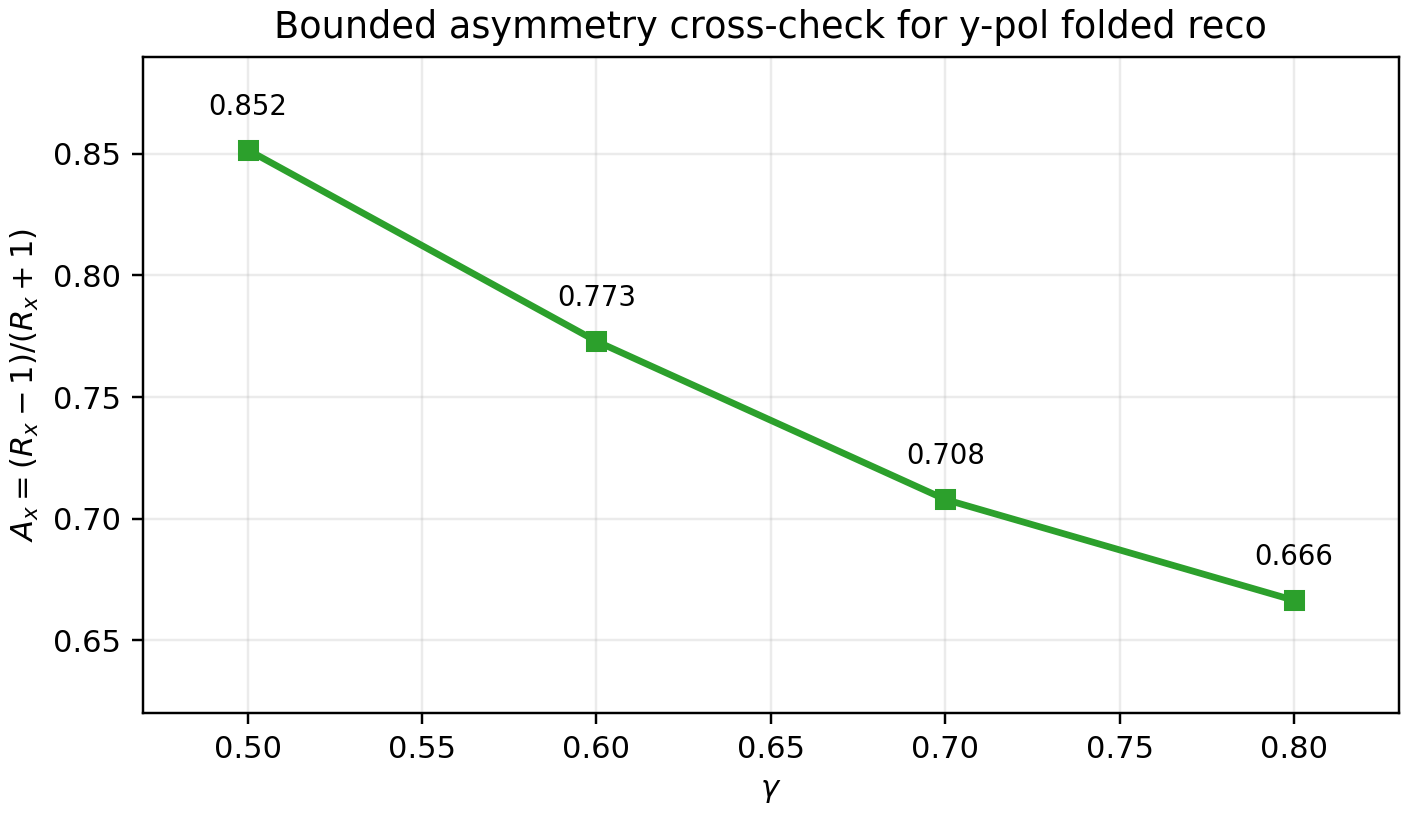
\includegraphics[width=0.74\linewidth]{ypol_bounded_asymmetry.png}

  \vspace{0.08cm}
  \scriptsize
  $\Ax$ is bounded and monotonic for the same reconstructed y-pol points.  It is
  a stability cross-check, not a replacement for the primary $R_x$ result.
\end{frame}

\begin{frame}{Backup D: Adjacent Gamma Separation}
  \scriptsize
  \begin{table}
    \centering
    \begin{tabular}{lrrrr}
      \toprule
      interval & $R_{\mathrm{left}}$ & $R_{\mathrm{right}}$ & $|\Delta R|$ & $N_{3\sigma}$ \\
      \midrule
      0.5$\to$0.6 & 12.48 & 7.81 & 4.67 & 519 \\
      0.6$\to$0.7 & 7.81 & 5.85 & 1.96 & 979 \\
      0.7$\to$0.8 & 5.85 & 4.99 & 0.85 & $2.77\times10^3$ \\
      \bottomrule
    \end{tabular}
  \end{table}
  \begin{block}{Scope}
    This is a planning-level statistical estimate. It is not an experimental
    significance claim because detector, polarization, background, and model
    systematics are not included.
  \end{block}
\end{frame}

\begin{frame}{Backup D: Usable-Event Survival}
  \begin{columns}[T,onlytextwidth]
    \begin{column}{0.56\textwidth}
      \centering
      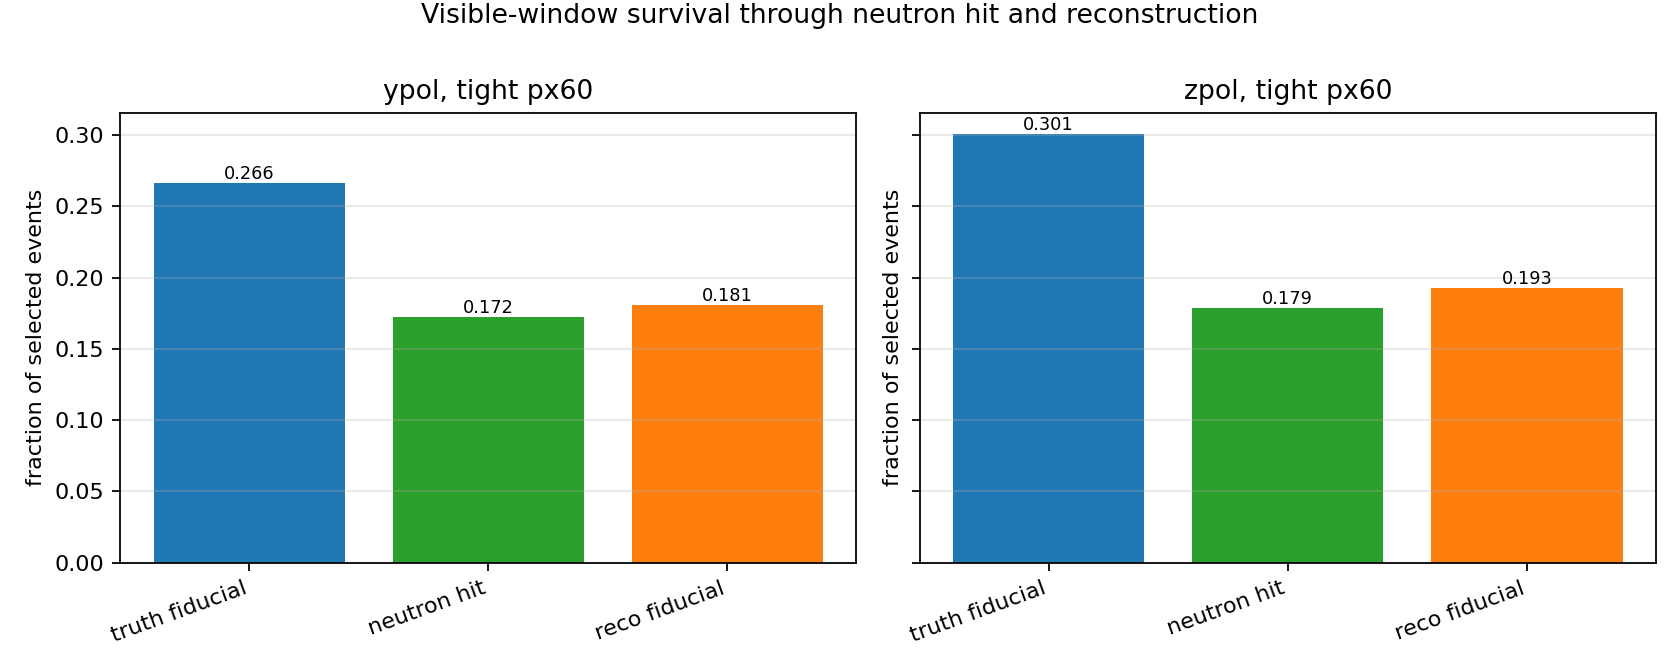
\includegraphics[width=\linewidth]{survival_flow_tight_px60.png}
    \end{column}
    \begin{column}{0.44\textwidth}
      \small
      Planning formula:
      \[
        N_{\mathrm{usable}}
        =
        \mathrm{rate}\times T\times
        \frac{N_{\mathrm{reco\ plane}}}{N_{\mathrm{raw}}}.
      \]
      For y-pol:
      \[
        \frac{N_{\mathrm{reco\ plane}}}{N_{\mathrm{raw}}}=0.00566
      \]
      \[
        N_{\mathrm{usable}}\simeq2.75\times10^5 .
      \]
    \end{column}
  \end{columns}
\end{frame}

\begin{frame}{Backup E: Sn112 and Other Targets}
  \begin{columns}[T,onlytextwidth]
    \begin{column}{0.50\textwidth}
      \centering
      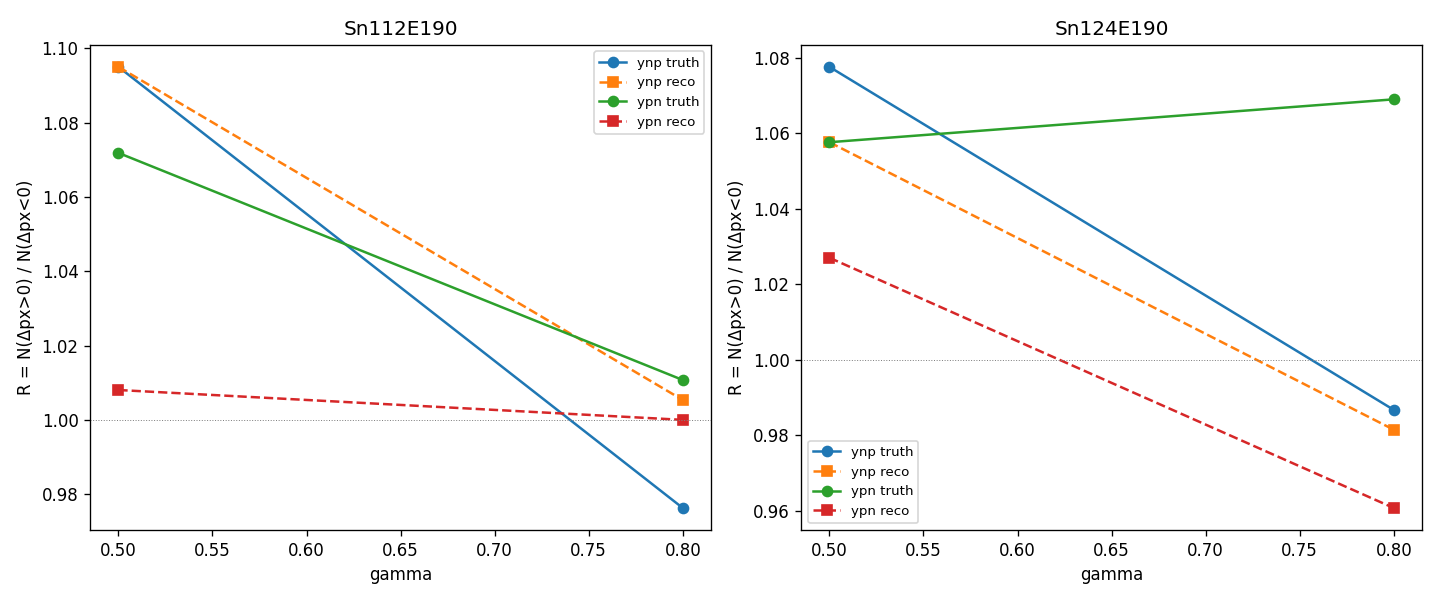
\includegraphics[width=\linewidth]{r_vs_gamma.png}
    \end{column}
    \begin{column}{0.50\textwidth}
      \small
      Sn112 is kept as an extension and cross-check target.
      \begin{itemize}
        \item The main body uses Sn124 because it is neutron-rich and has the
          most complete y-pol reconstruction sample.
        \item Target comparison should be folded and closed channel by channel
          before being combined.
      \end{itemize}
    \end{column}
  \end{columns}
\end{frame}

\begin{frame}{Backup E: z-pol Folded Results}
  \begin{columns}[T,onlytextwidth]
    \begin{column}{0.50\textwidth}
      \centering
      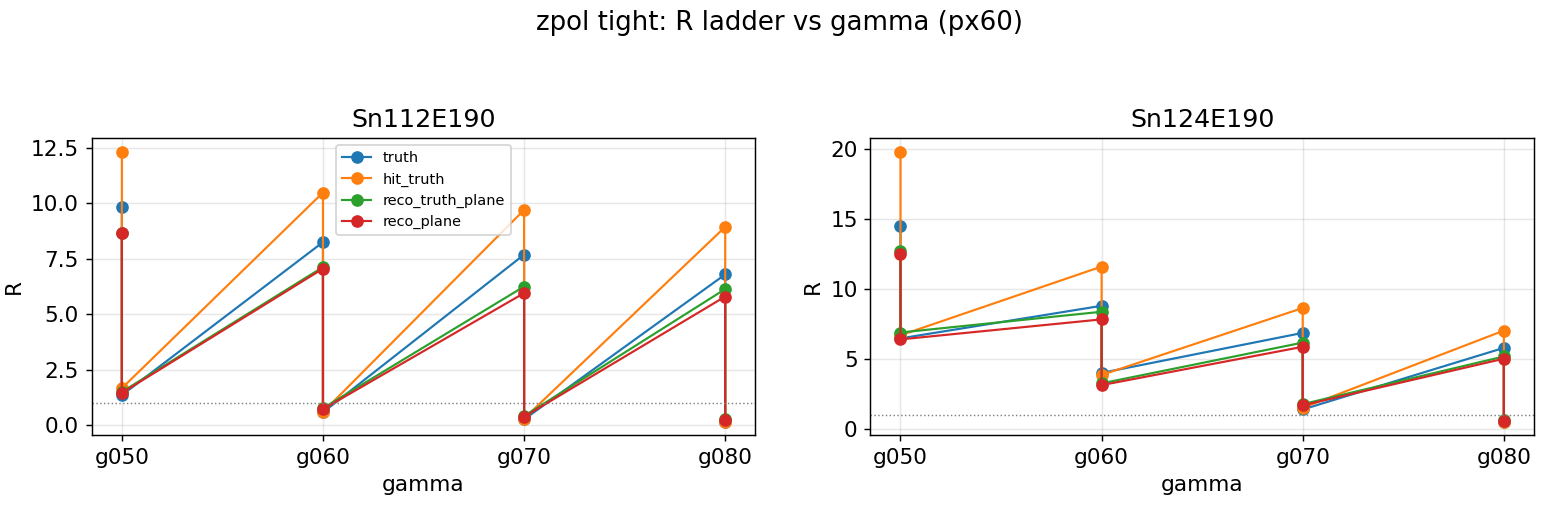
\includegraphics[width=\linewidth]{r_ladder_vs_gamma_zpol_tight_px60.png}
    \end{column}
    \begin{column}{0.50\textwidth}
      \scriptsize
      \begin{table}
        \centering
        \begin{tabular}{lrrr}
          \toprule
          $\gpar$ & $N_+$ & $N_-$ & $R_{\mathrm{reco}}$ \\
          \midrule
          0.5 & 306 & 48 & 6.38 \\
          0.6 & 208 & 67 & 3.10 \\
          0.7 & 214 & 129 & 1.66 \\
          0.8 & 171 & 307 & 0.56 \\
          \bottomrule
        \end{tabular}
      \end{table}
      z-pol remains useful for a second-stage experiment, but it is not part of
      the main y-pol baseline narrative.
    \end{column}
  \end{columns}
\end{frame}

\begin{frame}{Backup E: y-pol and z-pol Cut Definitions}
  \scriptsize
  \begin{columns}[T,onlytextwidth]
    \begin{column}{0.50\textwidth}
      \textbf{y-pol tight}
      \[
      |p_{y,p}^{\mathrm{truth}}-p_{y,n}^{\mathrm{truth}}|<150
      \]
      \[
      50<|\vec p_{T,p}^{\mathrm{truth}}+\vec p_{T,n}^{\mathrm{truth}}|<200
      \]
      \[
      \pi-|\phi_{\mathrm{truth}}|<0.2 .
      \]
    \end{column}
    \begin{column}{0.50\textwidth}
      \textbf{z-pol tight}
      \[
      p_{z,p}^{\mathrm{truth}}+p_{z,n}^{\mathrm{truth}}>1150
      \]
      \[
      |p_{z,p}^{\mathrm{truth}}-p_{z,n}^{\mathrm{truth}}|<150
      \]
      \[
      |\vec p_T^{\,\mathrm{sum}}|>50,\quad
      \pi-|\phi_{\mathrm{truth}}|<0.5 .
      \]
    \end{column}
  \end{columns}
  \vspace{0.12cm}
  All momenta are in MeV/$c$. These definitions are part of the current
  truth-assisted selection and must be migrated to reco-only cuts.
\end{frame}

\begin{frame}{Backup F: y-pol Polarization Monitoring}
  \begin{columns}[T,onlytextwidth]
    \begin{column}{0.50\textwidth}
      \centering
      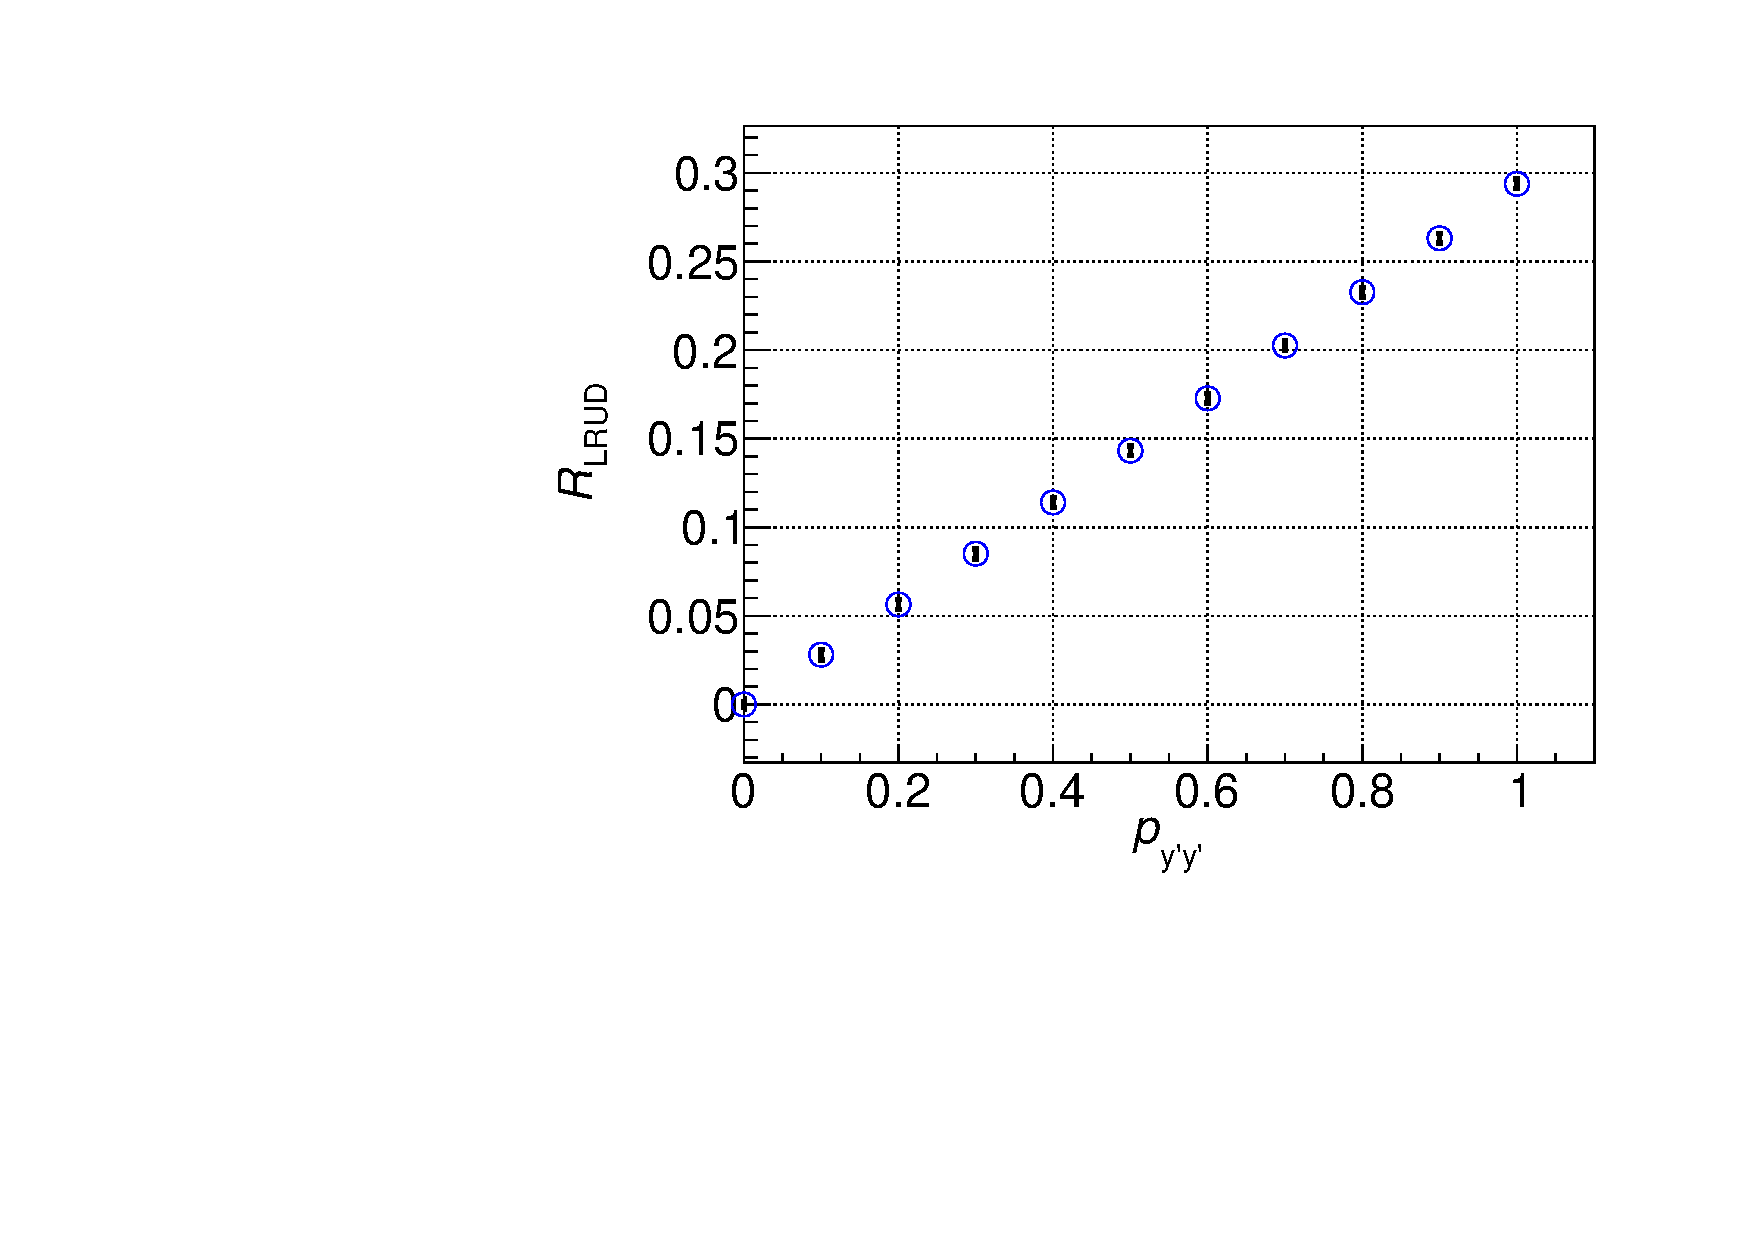
\includegraphics[width=0.95\linewidth]{R_LRUD_vs_pyy.pdf}
    \end{column}
    \begin{column}{0.50\textwidth}
      \small
      Vertical tensor polarization $p_{yy}$ can be monitored through an
      established azimuthal LRUD asymmetry in deuteron-proton elastic
      scattering.
      \begin{block}{Role in IVR}
        Polarization monitoring is an independent prerequisite for interpreting
        the IVR observable and must be propagated into $R_x(\gpar)$.
      \end{block}
    \end{column}
  \end{columns}
\end{frame}

\begin{frame}{Backup F: z-pol Monitoring Concept}
  \begin{columns}[T,onlytextwidth]
    \begin{column}{0.50\textwidth}
      \centering
      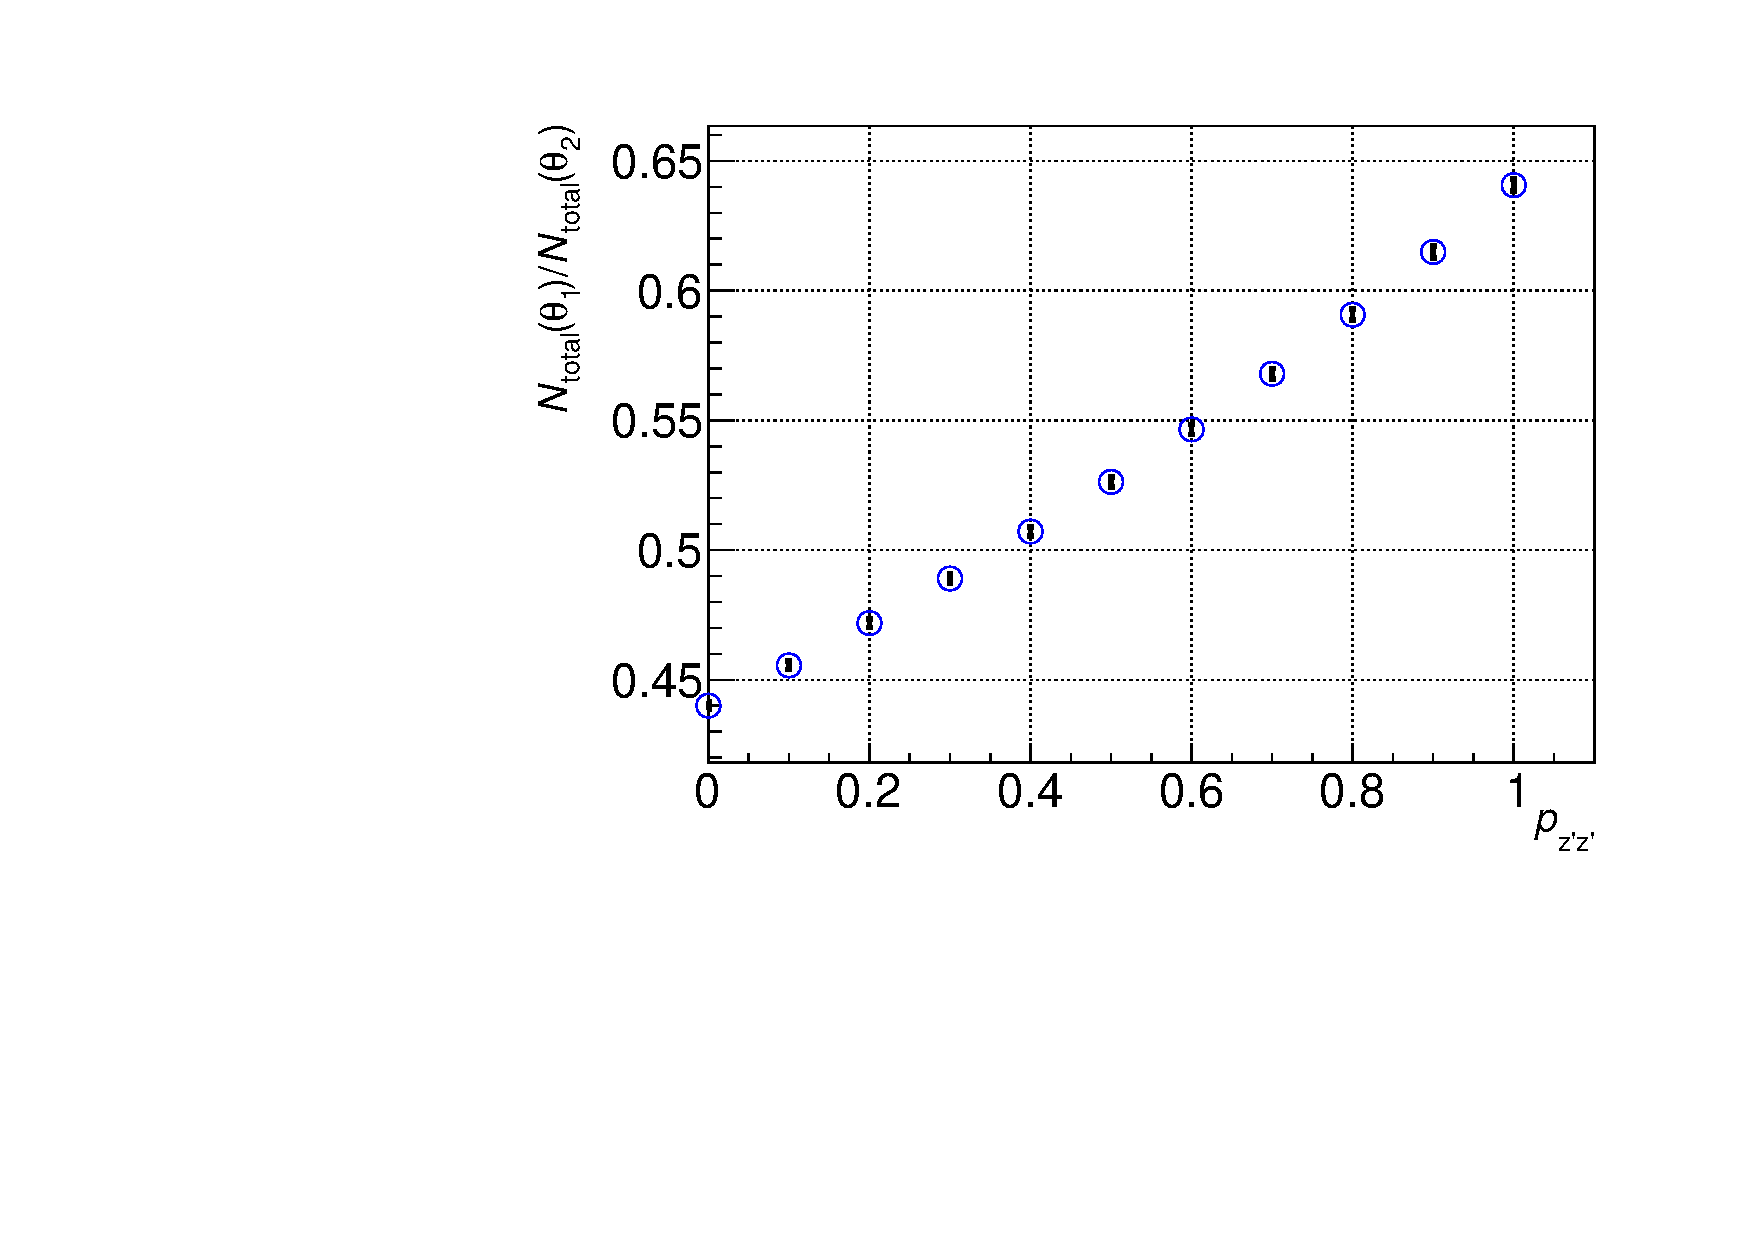
\includegraphics[width=0.95\linewidth]{Ratio_vs_pzz.pdf}
    \end{column}
    \begin{column}{0.50\textwidth}
      \small
      Longitudinal tensor polarization $p_{zz}$ can be monitored with a more
      demanding absolute/two-angle normalization strategy.
      \begin{block}{Careful statement}
        pzz monitoring is not impossible; it is a more complex second-stage
        requirement compared with the y-pol LRUD baseline.
      \end{block}
    \end{column}
  \end{columns}
\end{frame}

\begin{frame}{Backup G: Truth-Assisted Cuts}
  \small
  \begin{block}{What is fully reconstructed now}
    Numerator and denominator of $\Rcl$ use reconstructed proton momentum,
    reconstructed neutron momentum, and reconstructed event plane.
  \end{block}
  \begin{block}{What still uses truth}
    Event-quality cuts such as transverse balance and near-backscatter
    selection are currently defined using truth momenta in the simulation.
  \end{block}
  \begin{block}{Required closure}
    Re-run the same analysis with reco-only cuts and compare efficiency, purity,
    migration, and $\gpar$ ordering against the truth-assisted baseline.
  \end{block}
\end{frame}

\begin{frame}{Backup G: Detector-Systematic Checklist}
  \small
  \begin{itemize}
    \item neutron threshold, $T_0$, timing resolution, and hit-position model,
    \item cross-talk, fake neutron candidates, and accidental coincidences,
    \item charge-veto and charged-particle leakage assumptions,
    \item detector geometry and alignment variations,
    \item background and pile-up in the relevant electronics time window,
    \item polarization uncertainty and model/folding uncertainty.
  \end{itemize}
  \begin{block}{Next analysis product}
    Pseudo-data closure under detector and model variations, with the same
    folded comparison used for the experimental observable.
  \end{block}
\end{frame}

\end{document}
